\chapter{OUTPUT-BASED ERROR ESTIMATION AND MESH ADAPTATION
FOR VARIATIONAL MULTISCALE METHODS}
\label{chap:vms}

%%%%%%%%%%%%%%%%%%%%%%%%%%%%%%%%%%%%%%%%%%%%%%%%%%%%%%%%%%%%%%%%%%%%%%%%%%%%%%
\section{Introduction and motivation}
%%%%%%%%%%%%%%%%%%%%%%%%%%%%%%%%%%%%%%%%%%%%%%%%%%%%%%%%%%%%%%%%%%%%%%%%%%%%%%

Stabilized finite element methods have been used to
effectively solve a wide variety of problems where
standard Galerkin methods are known to be unstable.
Among these problems are the advective-diffusive
equations \cite{franca1992stabilized, hughes1989new},
Stokes flow \cite{hughes1986new, barth2004taxonomy},
and the Navier-Stokes equations \cite{brooks1982streamline,
franca1992stabilizedii, tezduyar1992incompressible}.
The variational multiscale (VMS) method, as developed
by Hughes et al. \cite{hughes1998variational,
hughes2007variational}, provides a systematic approach
to derive a stabilized finite element method. From
a high level, the VMS approach decomposes the solution
$u$ to a partial differential equation (PDE) into
\emph{coarse-scale} components $\bar{u}$ and
\emph{fine-scale} components $u'$,
where the fine-scale solution is represented or
approximated analytically.

\emph{A posteriori} error estimation is a common
tool to assess the accuracy and reliability of a
finite element solution \cite{ainsworth2011posteriori}.
In the original developments
of the VMS method, it was suggested that approximations
to the  fine-scale solution $u' = u - \bar{u}$
could be used to derive \emph{a posteriori} error
estimates \cite{hughes1998variational}. Since then,
numerous studies have utilized VMS techniques in
the context of \emph{a posteriori} error estimation.
Hauke et al. \cite{hauke2006multiscale, hauke2008variational}
investigated the using the fine-scale solution as
an explicit error estimator in the context
of advective transport problems. 
Masud et al. \cite{masud2011variational} derived explicit
and implicit error estimates for the global discretization
error for a mixed form of nearly incompressible elasticity,
and then later extended these techniques to nonlinear
elasticity formulations \cite{masud2013framework}.
Larson and M{\aa}lqvist
\cite{larson2007adaptive}
investigated approximating
the fine-scale solution via local patch-wise problems,
and derived an \emph{a posteriori} error estimate
for the solution in the energy norm for use in
an adaptive finite element method.

Traditional \emph{a posteriori} error estimates attempt
to bound the error in a given norm.
More recently developed duality-based \emph{a posteriori} error
estimates \cite{fidkowski2011review} seek to approximate
the error in an output quantity that can be expressed
as a functional $J(u)$. For example, outputs corresponding to
the lift or drag over an airfoil may be of primary
interest for a numerical study. In general, output-based
error estimates based on duality techniques require the
solution of an auxiliary \emph{dual problem}. In contrast,
the original PDE of interest is referred to as the
\emph{primal problem}. Using the solution $z$
to the dual problem, output error estimates are
written, in part, as the product
of two terms \cite{becker2001optimal, bangerth2013adaptive}.
The first term involves the residual $\R u^h$ of the
primal PDE evaluated at the finite element solution.
The second term, typically referred to as the
weighting term, involves the difference $z - I^h z$
between the exact dual solution and the nodal interpolant
of the exact dual solution onto the finite element space
used to approximate the primal problem.

The exact dual $z$ solution is generally unknown,
and thus must be approximated to obtain functional
error estimates. Note that if the dual solution is
approximated in the same finite element space as used
for the primal problem, then the weighting term in the
output error estimate is identically zero.
Thus some form of enrichment to the dual solution
is required. Several enrichment procedures are commonly
used. One approach is to approximate the exact dual
solution in a globally richer finite element space than
the one used for the primal problem. Another approach
involves solving the dual problem using the same finite
element space as used for the primal problem and enriching
the dual solution via projection. Yet another approach
involves using \emph{a priori} estimates to bound the
interpolation error in the dual solution.

In this paper we propose a novel strategy for output-based
error estimation, whereby the dual solution is enriched
by the \emph{fine-scale dual solution} $z'$ using VMS
techniques.
This is achieved by the introduction of a general
representation $\E_2$ for functional errors
in VMS methods. Using this general representation,
we introduce simple approximations to the fine and coarse
scale solutions for both the primal and dual problems to
derive an error estimate $\eta_2$.

We then seek to demonstrate the utility of this error
representation in adaptive finite elements.
This is achieved in part by comparison to a
recently proposed explicit output-based error representation
$\E_1$ that utilizes VMS techniques to
entirely circumvent the solution of an auxiliary dual problem
\cite{hauke2009variational}.
We prove that error estimates $\eta_1 \approx \E_1$
and $\eta_2 \approx \E_2$ based on this explicit error
representation and the newly proposed VMS technique, respectively,
are identical. However, we demonstrate that localization
of the explicit error estimate $\eta_1$ is
insufficient to drive mesh adaptation for \emph{local}
output quantities, whereas the estimate $\eta_2$
performs well.

The remainder of this paper is structured as follows.
We begin by presenting a review of the derivation
of a VMS method for an abstract Dirichlet primal problem.
Then we introduce simple approximations to the fine-scale
solution $u'$ and the coarse-scale solution $\bar{u}$
to obtain a computable numerical subgrid method for
the primal problem. Next, we introduce an auxiliary
dual problem to relate the output $J(u)$ to the primal
problem. We then derive a VMS and subgrid method for the
dual problem. Using the VMS methods for the primal and
dual problems, we derive a general expression $\E_2$ for
representing output errors in VMS methods, as well as
the previously proposed error representation $\E_1$.
Then, utilizing the approximations made for the primal
and dual subgrid models, we derive error estimates
$\eta_1 \approx \E_1$ and $\eta_2 \approx \E_2$
and demonstrate that these two quantities are identical.
Next, we discuss the localization of these error estimates
to element-level error indicators and how these indicators
are used to drive mesh adaptation procedures. Then we
investigate the effectivity of
error estimates $\eta_1$ and $\eta_2$ for one and
two dimensional example problems. We conclude by
investigating the ability of the estimates $\eta_1$
and $\eta_2$ to drive mesh adaptation to accurately
compute output quantities $J(u)$.

%%%%%%%%%%%%%%%%%%%%%%%%%%%%%%%%%%%%%%%%%%%%%%%%%%%%%%%%%%%%%%%%%%%%%%%%%%%%%%
\section{Review of VMS methods}
%%%%%%%%%%%%%%%%%%%%%%%%%%%%%%%%%%%%%%%%%%%%%%%%%%%%%%%%%%%%%%%%%%%%%%%%%%%%%%

%=============================================================================
\subsection{Model problem}
%=============================================================================

Let $\Omega \subset \mathbb{R}^d$
be an open bounded domain with smooth boundary
$\partial \Omega$, where $d$ is the number
of spatial dimensions of the domain. Let
$\V$ be a Hilbert space equipped with
the norm $\| \cdot \|_{\V}$ and inner product
$( \cdot, \cdot) _{\V}$ such that
$ \V = \{ u \in H(\Omega) : u|_{\partial \Omega} = 0 \} $,
where $H(\Omega)$ is a Hilbert space defined over
the domain $\Omega$.
Let $\V^*$ be the dual space of $\V$ and
$\pairb{\cdot}{\cdot}$ denote the dual pairing
between the two spaces given by
$\pairb{v}{u} = \int_{\Omega} v u \, \text{d} \Omega$.
Let $\OP : \V \to \V^*$
be a linear differential
operator. Let $f \in \V^*$ be given data.
We consider the abstract model problem of
finding $u \in \V$ such that
%
\begin{gather}
\begin{cases}
\begin{aligned}
\OP u &= f, & & \bs{x} \in \Omega, \\
u &= 0, & & \bs{x} \in \partial \Omega.
\end{aligned}
\end{cases}
\label{eq:primal_pde}
\end{gather}
%
In \ref{app:bcs} we discuss extending this model
problem to account for non-homogeneous Dirichlet and
Neumann boundary conditions.

We define the residual operator
$\R : \V \to \V^*$ as
$\R u:= f - \OP u$, and we refer to \eqref{eq:primal_pde}
as the \emph{primal problem}. The equivalent weak
form of the primal problem can be stated as:
find $u \in \V$ such that
%
\begin{gather}
\pairb{v}{\OP u} = \pairb{v}{f}
\quad \forall \, v \in \V.
\label{eq:primal_weak}
\end{gather}

%=============================================================================
\subsection{VMS formulation}
%=============================================================================

In this section, we review the foundations of the
VMS method, as developed by Hughes et al.
\cite{hughes1998variational} and later refined by
Hughes and Sangalli \cite{hughes2007variational}.
The basis of the method is the introduction
of a sum decomposition of the solution $u$ such
that $u = \bar{u} + u'$. Here $\bar{u} \in \bar{\V}$
corresponds to the computable \emph{coarse-scale}
solution, while $u' \in \V'$ is associated with
unresolved \emph{fine-scales} of the solution.
Further, it is assumed that the coarse-scale
space $\bar{\V}$ and fine-scale space $\V'$
are closed subspaces of $\V$ and that
$\bar{\V} \oplus \V' = \V$.

Using this sum decomposition, the weak form of the
primal problem can be restated: find
$\bar{u} + u' \in \V$ such that
%
\begin{gather}
\pairb{v}{\OP(\bar{u} + u')} = \pairb{v}{f}
\quad \forall \, v \in \V,
\label{eq:primal_weak_decomp}
\end{gather}
%
which can be split into the two subproblems:
find $\bar{u} + u' \in \V$ such that
%
\begin{gather}
\pairb{\bar{v}}{\OP \bar{u}} + \pairb{\bar{v}}{\OP u'} =
\pairb{\bar{v}}{f}
\quad \forall \, \bar{v} \in \bar{\V},
\label{eq:primal_subproblem_1}
\end{gather}
%
\begin{gather}
\pairb{v'}{\OP \bar{u}} + \pairb{v'}{\OP u'} =
\pairb{v'}{f}
\quad \forall \, v' \in \V'.
\label{eq:primal_subproblem_2}
\end{gather}

The goal of the VMS method
is to eliminate the fine-scale
solution $u'$ from the first sub-problem
\eqref{eq:primal_subproblem_1} by expressing
$u'$ in terms of the coarse-scale solution
$\bar{u}$. This results in a coarse-scale
model involving only $\bar{u}$ that can then
be solved numerically. However, the two sub-problems
are not currently well-posed in terms of uniqueness.
To ensure uniqueness, an optimality
condition $\phi(\cdot)$ is chosen, for example
$\phi(\cdot) = \| \cdot \|^2 _{H^1(\Omega)}$ or
$\phi(\cdot) = \| \cdot \|^2 _{L^2(\Omega)}$.
The problem is then reposed in the optimal
context:
%
\begin{gather}
\begin{aligned}
& \underset{\bar{u}}{\text{min}}
& & \phi(u-\bar{u}), \\
& \text{s.t.}
& & \begin{cases}
\bar{u} \in \bar{\V}, \\
u' \in \V', \\
\OP ( \bar{u} + u' ) = f,
\end{cases}
\end{aligned}
\label{eq:primal_optimality}
\end{gather}

The success of Hughes and Sangalli
\cite{hughes2007variational} is in showing
that this optimality criteria defines a
projector $\P : \V \to \bar{\V}$ onto the
coarse-scale space such that
$\P u' = 0$. Additionally, the projector $\P$
implicitly defines the fine-scale space
$\V' = \left\{ v \in \V \, : \, \P v = 0 \right\}$.
Using this projector, Hughes and Sangalli
then show that the fine-scale solution can
be analytically represented as:
%
\begin{gather}
u' = \underbrace{
\left(
\G - \G \P^T \left( \P \G \P^T \right) ^{-1} \P \G
\right)
}
_{\G'} \R \bar{u},
\label{eq:primal_fine_operator}
\end{gather}
%
where $\G = \OP^{-1}$ is the classical Green's
operator and $\G'$ is the so-called
\emph{fine-scale Green's operator}. Similarly,
the fine-scale solution can be written
in terms of the so-called
\emph{fine-scale Green's function} $g'(\bs{x};\bs{y})$
as
%
\begin{gather}
u'(\bs{y}) = \int_{\Omega} g'(\bs{x};\bs{y}) (\R \bar{u})(\bs{x})
\, \text{d} \Omega_x,
\label{eq:primal_fine_function}
\end{gather}
%
where $g'(\bs{x};\bs{y})$ is defined by the operator $\G'$.

Let $\OP^*$ be the adjoint operator of $\OP$ such that
%
\begin{gather}
\pairb{v}{\OP u} = \paira{\OP^* v}{u}
\quad \forall \, u, v \in \V.
\label{eq:adjoint}
\end{gather}
%
We note that this equation represents the definition of
the adjoint operator $\OP^*$ and does not place any
restriction on $\OP$. When $\OP$ is self adjoint, we
have the identity $\OP^* = \OP$, otherwise $\OP^*$
and $\OP$ are different. However, equation
\eqref{eq:adjoint} holds in either case.

Using the definition of the adjoint \eqref{eq:adjoint}
and the representation of the
fine-scale solution \eqref{eq:primal_fine_operator},
the first sub-problem \eqref{eq:primal_subproblem_1}
can be restated as:
find $\bar{u} \in \bar{V}$ such that
%
\begin{gather}
\pairb{\bar{v}}{\OP \bar{u}} +
\paira{\OP^* \bar{v}}{\G' \R \bar{u}} =
\pairb{\bar{v}}{f}
\quad \forall \, \bar{v} \in \bar{\V}.
\label{eq:primal_vms}
\end{gather}
%
We refer to this equation as the \emph{continuous
variational multiscale} formulation of the primal
problem. For use in later derivations, we rewrite
this formulation as:
%
\begin{gather}
\paira{\OP^* \bar{v}}{\G' \R \bar{u}} = \pairb{\bar{v}}{\R \bar{u}}
\quad \forall \, \bar{v} \in \bar{\V},
\label{eq:primal_vms_2}
\end{gather}
%
recalling the definition of the primal residual
operator $\R u:= f - \OP u$.

%=============================================================================
\subsection{Subgrid model}
%=============================================================================

In practice, the continuous VMS model
\eqref{eq:primal_vms} is approximated by a finite
element method. We refer to this approximate
model as the \emph{subgrid model}, as is common
in the literature. The first step in this
approximation is to choose the coarse-scale space to be
a finite dimensional subspace, that is
$\bar{\V} = \V^h$, and partition the domain
$\Omega$ into $n_{el}$ non-overlapping finite
element subdomains $\Omega^e$ with boundaries
$\partial \Omega^e$ for $e=1,2,\dots,n_{el}$.

Next we note that an exact representation for the
fine-scale Green's function $g'(\bs{x};\bs{y})$ (and
the fine-scale Green's operator $\G'$) is
generally not obtainable. Thus, we must introduce
an approximation for the fine-scale Green's function
to accurately represent the fine-scale solution
\eqref{eq:primal_fine_function}. To this end, we
introduce the so-called \emph{element-level Green's
function} $g^e(\bs{x};\bs{y})$, defined over element
interiors as
%
\begin{gather}
\begin{cases}
\begin{aligned}
\OP^* g^e(\bs{x}; \bs{y}) &= \delta(\bs{x} - \bs{y}),
\quad & & \bs{x} \in \Omega^e, \\
g^e(\bs{x}; \bs{y}) &= 0, \quad & & \bs{x} \in \partial \Omega^e,
\end{aligned}
\end{cases}
\label{eq:primal_elem_greens}
\end{gather}
such that $g'(\bs{x};\bs{y}) \approx g^e(\bs{x};\bs{y})$.

Note that this approximation assumes that the
fine-scale solution $u'$ vanishes on element boundaries
$\partial \Omega^e$. Hughes and Sangalli
\cite{hughes2007variational} show that, in one spatial
dimension, the choice of an $H^1$ optimality
condition $\phi = \| \cdot \|^2_{H^1}$ results
in a completely \emph{local} fine-scale Green's
function. That is, when $d = 1$, the $H^1$
optimality condition ensures the equivalence
of the fine-scale Green's function
$g'(\bs{x};\bs{y})$ and the element-level Green's function
$g^e(\bs{x};\bs{y})$. This result provides justification
for approximating the fine-scale Green's function
as the element-level Green's function and motivates
us to only consider $\phi(\cdot) = \| \cdot \|_{H^1}$
in this work.

As a further simplification, we approximate the
element-level Green's function by it's \emph{average}
value over the element interior, and denote this
value by $\uptau^e$, which can be expressed as:
%
\begin{gather}
\uptau^e = \frac{1}{\text{meas}(\Omega^e)}
\int_{\Omega^e} \, \int_{\Omega^e}
g^e (\bs{x}; \bs{y}) \, \text{d} \Omega_x \, \text{d} \Omega_y.
\label{eq:primal_tau}
\end{gather}
%
We note that more accurate approximations for the
element-level Green's function can be made. For instance,
Oberai and Pinsky \cite{oberai1998multiscale} approximate
the element-level Green's function by a polynomial scalar
function involving \emph{moments} of the element-level
Green's function. We leave investigation into this area
as a consideration for future work.

With this final approximation, the subgrid model
can be written as: find $u^h \in \V^h$ such that
%
\begin{gather}
\pairb{v^h}{\OP u^h} +
\paira{\OP^* v^h}{\uptau^e \R u^h}^{\Omega'} =
\pairb{v^h}{f}
\quad \forall \, v^h \in \V^h,
\label{eq:primal_subgrid}
\end{gather}
%
or equivalently as: find $u^h \in \V^h$ such that
%
\begin{gather}
\paira{\OP^* v^h}{\uptau^e \R u^h}^{\Omega'} =
\pairb{v^h}{\R u^h} \quad \forall \, v^h \in \V^h,
\label{eq:primal_subgrid_2}
\end{gather}
%
where we have approximated the fine-scale solution
over element interiors as
%
\begin{gather}
u' \bigr|_{\Omega^e} \approx
\tilde{u}' \bigr|_{\Omega^e} =
\uptau^e \R u^h.
\label{eq:primal_fine_approx}
\end{gather}
%
Here $\paira{\cdot}{\cdot}^{\Omega'}$ denotes the `broken'
dual pairing over element interiors given by
%
\begin{gather}
\paira{u}{v}^{\Omega'} = 
\sum_{e=1}^{n_{el}} \paira{u}{v}^{\Omega^e},
\end{gather}
where we have denoted the dual pairing over a single
element interior as
%
\begin{gather}
\paira{u}{v}^{\Omega^e} =
\int_{\Omega^e} u v \, \text{d} \Omega.
\end{gather}

We emphasize that the approximations
made to the fine-scale solution imply that
the subgrid model \eqref{eq:primal_subgrid}
is an approximation to the continuous VMS
formulation \eqref{eq:primal_vms}, which in turn
implies that the subgrid solution $u^h$ is
an approximation to the coarse-scale
solution $\bar{u}$. With this in mind, we
can express the exact solution $u$ as
%
\begin{gather}
u = u^h + \tilde{u}' + \tilde{u}
\label{eq:primal_subgrid_decomp}
\end{gather}
%
where $\tilde{u} = (\bar{u} - u^h) + (u' - \tilde{u}')$
represents the approximation errors in the coarse
and fine-scale solutions.

\begin{rmk}
The finite element method is derived from the weak
form of a partial differential equation that has
been integrated by parts. Thus instead
of the duality pairing used in equation \eqref{eq:primal_subgrid}
it makes use of the $L_2$ inner product, and the finite
element subgrid model derived from the variational
multiscale method is given by:
%
\begin{gather}
A(v^h, u^h) + (\OP^* v^h, \uptau^e \R u^h)_{\Omega'} = l(v^h)
\quad \forall \, v \in \V.
\label{eq:primal_fem}
\end{gather}
%
where $A(\cdot, \cdot)$ is the bilinear form associated with
the operator $\OP$, $(\cdot, \cdot)_{\Omega'}$ is the broken
$L_2$ inner product defined on element interiors, and
$l(\cdot)$ is the linear functional associated with the forcing
function $f$.
\end{rmk}

%%%%%%%%%%%%%%%%%%%%%%%%%%%%%%%%%%%%%%%%%%%%%%%%%%%%%%%%%%%%%%%%%%%%%%%%%%%%%%
\section{The dual problem}
%%%%%%%%%%%%%%%%%%%%%%%%%%%%%%%%%%%%%%%%%%%%%%%%%%%%%%%%%%%%%%%%%%%%%%%%%%%%%%

%=============================================================================
\subsection{Abstract problem}
%=============================================================================

Let $J(u) : \V \to \mathbb{R}$ be a linear functional
corresponding to a physically meaningful quantity of
interest. We assume that $J(u)$ can be expressed as
%
\begin{gather}
J(u) = \paira{q}{u},
\label{eq:functional}
\end{gather}
%
where $q \in \V^*$. Following standard duality-based
approaches for \emph{a posteriori} error estimation
\cite{bangerth2013adaptive, becker2001optimal,
eriksson1995introduction, fidkowski2011review}
we introduce the \emph{dual problem} : find $z \in \V$
such that
%
\begin{gather}
\paira{\OP^* z}{v} = \paira{q}{v}
\quad \forall \, v \in \V.
\label{eq:dual_weak}
\end{gather}
%
The equivalent strong form of the dual problem can be written
as: find $z \in \V$ such that
%
\begin{gather}
\begin{cases}
\begin{aligned}
\OP^* z &= q, \quad & & \bs{x} \in \Omega, \\
z &= 0, \quad & & \bs{x} \in \partial \Omega.
\end{aligned}
\end{cases}
\label{eq:dual_pde}
\end{gather}
%
We define the residual operator
$\R^* : \V \to \V^*$ of the dual problem as
$\R^* z := q - \OP^* z$.

%=============================================================================
\subsection{VMS formulation}
%=============================================================================

If the primal problem necessitates the use of numerical
stabilization, it is also likely that solving the dual problem
\eqref{eq:dual_weak} with a Galerkin finite element method will
yield spurious oscillations in the dual solution
\cite{cyr2014approaches}. To prevent non-physical behavior
in the dual solution, we also solve the dual problem with a VMS
method. Cyr et al. \cite{cyr2014approaches} call this
approach the \emph{stabilization of the adjoint}. This is in
contrast to deriving a dual problem directly from the primal
subgrid model \eqref{eq:primal_subgrid}, which Cyr et al.
refer to as the \emph{adjoint of the stabilization}.

Let $\bar{\V}_d$ and $\V'_d$ be closed subspaces of $\V$.
Obtaining a VMS formulation for the dual problem proceeds
in exactly the same manner as the primal problem. First
a sum decomposition of the dual solution $z$ is assumed
such that $z = \bar{z} + z'$, where $\bar{z} \in \bar{\V}_d$
and $z' \in \V'_d$. The weak form of the dual problem
\eqref{eq:dual_weak} is then written as two sub-problems,
whose solutions are uniquely determined by an optimality
condition $\phi_d(\cdot)$ imposed on the coarse-scale
solution $\bar{z}$. As with the primal model, we will only
consider the $H^1$ optimality condition
$\phi_d(\cdot) = \| \cdot \|^2_{H^1}$. However, we note
that one could potentially choose different optimality
conditions for both the primal and dual problems. We leave
investigation into this area as an open research topic.

The optimality condition defines a projector
$\P_d : \V \to \bar{\V}_d$ onto the coarse-scale subspace
such that $P_d z' = 0$, and this projector implicitly
defines the fine-scale subspace as
$\bar{\V}_d = \{ v \in \V \, : \, \P_d v = 0 \}$. If we
let $\G_d$ denote the classical Green's operator for
the dual problem, such that $\G_d = (\OP^*)^{-1}$, then
the fine-scale dual solution can be represented as:
%
\begin{gather}
z' = \underbrace{
\left(
\G_d - \G_d \P_d^T \left( \P_d \G_d \P_d^T \right) ^{-1} \P_d \G_d
\right)
}
_{\G'_d} \R^* \bar{z},
\label{eq:dual_fine_operator}
\end{gather}
%
where $\G'_d$ is the \emph{dual fine-scale Green's operator}.
Similarly, the fine-scale solution can be written in terms
of the \emph{dual fine-scale Green's function}, $g'_d(\bs{x};\bs{y})$,
as:
%
\begin{gather}
z'(\bs{y}) = \int_{\Omega} g'_d(\bs{x};\bs{y}) (\R^* \bar{z})(\bs{x})
\, \text{d} \Omega_x,
\label{eq:dual_fine_function}
\end{gather}
where $g'_d(\bs{x};\bs{y})$ is defined by the operator $\G'_d$.
Using this representation of the fine-scale dual solution,
the \emph{continuous variational multiscale} formulation of
the dual problem is stated as: find $\bar{z} \in \bar{\V}_d$
such that
%
\begin{gather}
\paira{\OP^* \bar{z}}{\bar{v}} +
\pairb{\G'_d \R^* \bar{z}}{\OP \bar{v}} =
\paira{q}{\bar{v}}
\quad \forall \, \bar{z} \in \bar{\V}_d.
\label{eq:dual_vms}
\end{gather}
%
Recalling the definition of the dual residual operator
$\R^* := q - \OP^*$, we can rewrite equation \eqref{eq:dual_vms}
as:
%
\begin{gather}
\pairb{\G'_d \R^* \bar{z}}{\OP \bar{v}} =
\paira{\R^* \bar{z}}{\bar{v}}
\quad \forall \, \bar{z} \in \bar{\V}_d.
\label{eq:dual_vms_2}
\end{gather}
%

%=============================================================================
\subsection{Subgrid model}
%=============================================================================

To derive a corresponding subgrid model to the VMS formulation
of the dual problem \eqref{eq:dual_vms}, we will assume that the
coarse-scale spaces for the primal and dual problem are chosen
to be the same, such that $\bar{\V} = \bar{\V}_d$. Additionally, we will
consider approximations made using the same finite dimensional subspace
$\bar{\V} = \V^h$ and discretization as used for the primal
subgrid model. We first approximate the dual fine-scale Green's
function $g'_d(\bs{x};\bs{y})$ using the \emph{dual element-level
Green's function}, defined over element interiors as
%
\begin{gather}
\begin{cases}
\begin{aligned}
\OP g^e_d(\bs{x}; \bs{y}) &= \delta(\bs{x} - \bs{y}),
\quad & & \bs{x} \in \Omega^e, \\
g^e_d(\bs{x}; \bs{y}) &= 0, \quad & & \bs{x} \in \partial \Omega^e,
\end{aligned}
\end{cases}
\label{eq:dual_elem_greens}
\end{gather}
%
such that $g'_d(\bs{x};\bs{y}) \approx g^e_d(\bs{x};\bs{y})$.

We further approximate the fine-scale dual solution $z'$
by writing it as the product of a scalar function $\uptau^e_d$
times the dual residual operating on the coarse-scale solution.
The scalar function is given as:
%
\begin{gather}
\uptau^e_d = \frac{1}{\text{meas}(\Omega^e)}
\int_{\Omega^e} \, \int_{\Omega^e}
g^e_d(\bs{x}; \bs{y}) \, \text{d} \Omega_x \, \text{d} \Omega_y.
\label{eq:dual_tau}
\end{gather}
%
The dual subgrid model can then be written as: find $z^h \in \V^h$
such that
%
\begin{gather}
\paira{\OP^* z^h}{v^h} +
\pairb{\uptau^e_d \R^* z^h}{\OP v^h}^{\Omega'} =
\paira{q}{v^h}
\quad \forall \, v^h \in \V^h,
\label{eq:dual_subgrid}
\end{gather}
%
or equivalently as: find $z^h \in \V^h$ such that
%
\begin{gather}
\pairb{\uptau^e_d \R^* z^h}{\OP v^h}^{\Omega'} =
\paira{\R^* z^h}{v^h}
\quad \forall \, v^h \in \V^h,
\label{eq:dual_subgrid_2}
\end{gather}
where we have approximated the fine-scale dual solution over
element interiors as
%
\begin{gather}
z' \bigr|_{\Omega^e} \approx
\tilde{z}' \bigr|_{\Omega^e} =
\uptau^e_d \R^* z^h.
\label{eq:dual_fine_approx}
\end{gather}
%
We note that the exact dual solution can be
expressed as the sum
%
\begin{gather}
z = z^h + \tilde{z}' + \tilde{z},
\label{eq:dual_subgrid_decomp}
\end{gather}
%
where $\tilde{z} = (\bar{z} - z^h) + (z' - \tilde{z}')$
represents the approximation errors in the coarse and
fine-scale solutions.

\begin{rmk}
The finite element version of the dual subgrid model
corresponding to equation \eqref{eq:dual_subgrid} is
written using the $L_2$ inner product as:
%
\begin{gather}
A(z^h, v^h) + (\uptau^e_d \R^* z^h, \OP v^h)_{\Omega'} = J(v^h)
\quad \forall \, v \in \V^h,
\label{eq:dual_fem}
\end{gather}
%
where $A(\cdot, \cdot)$ is the bilinear form associated with
the operator $\OP$, and $(\cdot, \cdot)_{\Omega'}$ is the broken
$L_2$ inner product defined on element interiors.
\end{rmk}

%%%%%%%%%%%%%%%%%%%%%%%%%%%%%%%%%%%%%%%%%%%%%%%%%%%%%%%%%%%%%%%%%%%%%%%%%%%%%%
\section{Error estimation}
\label{sec:Error}
%%%%%%%%%%%%%%%%%%%%%%%%%%%%%%%%%%%%%%%%%%%%%%%%%%%%%%%%%%%%%%%%%%%%%%%%%%%%%%

In this section, we develop a general framework for output-based
error estimation in VMS methods. We first develop two error
representations for output quantities in the continuous VMS setting.
Next, we discuss the role of the approximations made in both the
primal and dual subgrid models. Finally, we introduce two error
estimates for output quantities. We prove that the error estimates
are identical. However, we demonstrate the superiority of one
estimate over the other in the context of error localization needed
to drive mesh adaptation.

%=============================================================================
\subsection{Continuous VMS error representations}
%=============================================================================

\begin{prop}
For any solution $u = u' + \bar{u}$ to the continuous VMS
formulation \eqref{eq:primal_vms}, we have the error representation
%
\begin{gather}
\E_1 = J(u) - J(\bar{u}) = J(u')
\end{gather}
%
\end{prop}

\begin{proof}
The result follows directly from the linearity of $J(\cdot)$ and
the sum decomposition $u = u' + \bar{u}$.
\end{proof}

This error representation is used by Hauke and Fuster
\cite{hauke2009variational} to derive an explicit
\emph{a posteriori} error estimate for output quantities.
The error estimate only involves an approximation
$\tilde{u}'$ to the fine-scale solution $u'$ and
completely avoids the solution of a dual problem.
However, when $q$ is chosen to be a \emph{local}
forcing function for the dual problem (e.g. a function
which is non-zero only over a subdomain of the total
domain), error estimates derived from this
representation fail to provide useful information
when they are localized to the element level.
Such error localization is critical to drive
mesh adaptation and is discussed in detail later.

\begin{prop}
For any solutions $u = u' + \bar{u}$ to the continuous VMS
formulation \eqref{eq:primal_vms} and $z = z' + \bar{z}$ to the
continuous dual VMS formulation \eqref{eq:dual_vms}, we have the
error representation
%
\begin{gather}
\E_2 = J(u) - J(\bar{u}) =
\pairb{\G'_d \R^* \bar{z}}{ \R \bar{u}} +
\paira{\OP^* \bar{z}}{\G' \R \bar{u}}
\label{eq:error_cont_1}
\end{gather}
%
\end{prop}

\begin{proof}
%
\begin{gather*}
\begin{aligned}
J(u) - J(\bar{u}) &=
\paira{q}{u} - \paira{q}{\bar{u}}
&& \text{by \eqref{eq:functional}} \\
&= \paira{\OP^* z}{u} - \paira{\OP^* z}{\bar{u}}
&& \text{by \eqref{eq:dual_weak}} \\
&= \pairb{z}{\OP u} - \pairb{z}{\OP \bar{u}}
&& \text{by \eqref{eq:adjoint}} \\
&= \pairb{z}{f} - \pairb{z}{\OP \bar{u}}
&& \text{by \eqref{eq:primal_weak}} \\
&= \pairb{z}{\R \bar{u}}
&& \text{by definition, linearity} \\
&= \pairb{z'}{\R \bar{u}} + \pairb{\bar{z}}{\R \bar{u}}
&& \text{by definition, linearity} \\
&= \pairb{z'}{\R \bar{u}} + \paira{\OP^* \bar{z}}{\G' \R \bar{u}}
&& \text{by \eqref{eq:primal_vms_2}} \\
&= \pairb{\G'_d \R^* \bar{z}}{\R \bar{u}} +
\paira{\OP^* \bar{z}}{\G' \R \bar{u}}
&& \text{by \eqref{eq:dual_fine_operator}}
\end{aligned}
\label{eq:error_cont_2}
\end{gather*}
\end{proof}

This error representation suggests a general approach
to output-based error estimation for VMS methods, where
the only approximation made to this point is that the
coarse-scale subspace for the primal and dual problems
are equal, such that $\bar{\V} = \bar{\V}_d$. To derive
computable error estimates, exact representations or
approximations must be known for the fine-scale
Green's operators and the coarse-scale solutions for
both the primal and dual problems.

%=============================================================================
\subsection{Subgrid model error representations}
%=============================================================================

We now derive error representations that arise by
introducing the approximations made in the primal
and dual subgrid models.

\begin{prop}
For any solutions $u$ to the primal model \eqref{eq:primal_weak}
and $u^h$ to the primal subgrid model \eqref{eq:primal_subgrid},
we have the error representation
%
\begin{gather}
\hat{\E}_1 = J(u) - J(u^h) =
\paira{q}{\uptau^e \R u^h}^{\Omega'} + \paira{q}{\tilde{u}}
\label{eq:representation_1}
\end{gather}
%
\end{prop}

\begin{proof}
%
\begin{gather*}
\begin{aligned}
J(u) - J(u^h) &=
\paira{q}{u} - \paira{q}{u^h}
&& \text{by \eqref{eq:functional}} \\
&= \paira{q}{u - u^h}
&& \text{by linearity} \\
&= \paira{q}{\tilde{u}' + \tilde{u}}
&& \text{by \eqref{eq:primal_subgrid_decomp}} \\
&= \paira{q}{\tilde{u}'}^{\Omega'} + \paira{q}{\tilde{u}}
&& \text{by linearity} \\
&= \paira{q}{\uptau^e \R u^h}^{\Omega'} + \paira{q}{\tilde{u}}
&& \text{by \eqref{eq:primal_fine_approx}} \\
\end{aligned}
\end{gather*}
%
\end{proof}

\begin{prop}
For any solutions $u$ to the primal model \eqref{eq:primal_weak},
$z$ to the dual model \eqref{eq:dual_weak}, $u^h$ to the primal
subgrid model \eqref{eq:primal_subgrid} and $z^h$ to the dual
subgrid model \eqref{eq:dual_subgrid}, we have the error
representation
%
\begin{gather}
\begin{aligned}
\hat{\E}_2 &= J(u) - J(u^h) \\
&=
\pairb{\uptau^e_d \R^* z^h}{\R u^h}^{\Omega'} +
\paira{\OP^* z^h}{\uptau^e \R u^h}^{\Omega'} +
\pairb{\tilde{z}}{\R u^h}
\end{aligned}
\label{eq:representation_2}
\end{gather}
%
\end{prop}

\begin{proof}
\begin{gather*}
\begin{aligned}
&J(u) - J(u^h) \\
&=
\paira{q}{u} - \paira{q}{u^h}
&& \text{by \eqref{eq:functional}} \\
&=
\paira{\OP^* z}{u} - \paira{\OP^* z}{u^h}
&& \text{by \eqref{eq:dual_weak}} \\
& =
\pairb{z}{\OP u} - \pairb{z}{\OP u^h}
&& \text{by \eqref{eq:adjoint}} \\
&=
\pairb{z}{f} - \pairb{z}{\OP u^h}
&& \text{by \eqref{eq:primal_weak}} \\
&=
\pairb{z}{\R u^h}
&& \text{by definition} \\
&=
\pairb{z}{\R u^h} - \pairb{z^h}{\R u^h} +
\paira{\OP^* z^h}{\uptau^e \R u^h}^{\Omega'}
&& \text{by \eqref{eq:primal_subgrid_2}} \\
&=
\pairb{z - z^h}{\R u^h} +
\paira{\OP^* z^h}{\uptau^e \R u^h}^{\Omega'}
&& \text{by linearity} \\
&=
\pairb{\tilde{z}' + \tilde{z}}{\R u^h} +
\paira{\OP^* z^h}{\uptau^e \R u^h}^{\Omega'}
&& \text{by \eqref{eq:dual_subgrid_decomp}} \\
&=
\pairb{\tilde{z}'}{\R u^h}^{\Omega'} +
\paira{\OP^* z^h}{\uptau^e \R u^h}^{\Omega'} +
\pairb{\tilde{z}}{ \R u^h}
&& \text{by linearity} \\
&=
\pairb{\uptau^e_d \R^* z^h}{\R u^h}^{\Omega'} +
\paira{\OP^* z^h}{\uptau^e \R u^h}^{\Omega'} +
\pairb{\tilde{z}}{ \R u^h}
&& \text{by \eqref{eq:dual_fine_approx}}
\end{aligned}
\end{gather*}
\end{proof}

%=============================================================================
\subsection{Subgrid model error estimates}
%=============================================================================

In general, the approximation errors $\tilde{u}$
and $\tilde{z}$ are unknown. This suggests the
error \emph{estimates} $\eta_1 \approx \hat{\E}_1$
and $\eta_2 \approx \hat{\E}_2$ that are obtained
by setting $\tilde{u} = 0$ in \eqref{eq:representation_1}
and $\tilde{z} = 0$ in \eqref{eq:representation_2}, and
are given below:
%
\begin{gather}
\eta_1 = \paira{q}{\uptau^e \R u^h}^{\Omega'}
\label{eq:estimate_1}
\end{gather}
%
\begin{gather}
\eta_2 =
\pairb{\uptau^e_d \R^* z^h}{\R u^h}^{\Omega'} +
\paira{\OP^* z^h}{\uptau^e \R u^h}^{\Omega'}
\label{eq:estimate_2}
\end{gather}

\begin{prop}
For any solutions $u^h$ to the primal subgrid model
\eqref{eq:primal_subgrid} and $z^h$ to the dual
subgrid model \eqref{eq:dual_subgrid} the error estimates
$\eta_1$ and $\eta_2$ are identical.
\end{prop}

\begin{proof}
Note that if the stabilization parameters $\uptau^e$ and
$\uptau^e_d$ for the primal and dual problems are equal,
we obtain the desired result since
%
\begin{gather*}
\begin{aligned}
\eta_2 &= 
\pairb{\uptau^e_d \R^* z^h}{\R u^h}^{\Omega'} +
\paira{\OP^* z^h}{\uptau^e \R u^h}^{\Omega'}
&&\\
&= \paira{\R^* z^h}{\uptau^e \R u^h}^{\Omega'} +
\paira{\OP^* z^h}{\uptau^e \R u^h}^{\Omega'}
&&\text{by assumption} \\
&= \paira{\R^* z^h + \OP^* z^h}{\uptau^e \R u^h}^{\Omega'}
&&\text{by linearity} \\
&= \paira{q}{\uptau^e \R u^h}^{\Omega'}
&&\text{by definition} \\
&= \eta_1
&&
\end{aligned}
\end{gather*}
%
Using the given definitions \eqref{eq:primal_tau}
and \eqref{eq:dual_tau}, we note that a sufficient
condition for the equality $\uptau^e = \uptau^e_d$
is:
$g^e(\bs{x}; \bs{y}) = g^e_d(\bs{y}; \bs{x})$.
This is verified via the following argument:
%
\begin{gather*}
\begin{aligned}
\OP^* g^e(\bs{x}; \bs{y})
&=
\delta(\bs{x} - \bs{y})
&& \text{by \eqref{eq:primal_elem_greens}} \\
\implies
\int_{\Omega^e}
g^e_d(\bs{x}; \bs{z}) \OP^* g^e(\bs{x}; \bs{y})
\, \text{d} \Omega
&=
\int_{\Omega^e}
g^e_d(\bs{x}; \bs{z}) \delta(\bs{x} - \bs{y})
\, \text{d} \Omega
&& \\
\implies
\int_{\Omega^e}
\OP g^e_d(\bs{x}; \bs{z}) g^e(\bs{x}; \bs{y})
\, \text{d} \Omega
&=
\int_{\Omega^e}
g^e_d(\bs{x}; \bs{z}) \delta(\bs{x} - \bs{y})
\, \text{d} \Omega
&& \\
\implies
\int_{\Omega^e}
\delta(\bs{x} - \bs{z}) g^e(\bs{x}; \bs{y})
\, \text{d} \Omega
&=
\int_{\Omega^e}
g^e_d(\bs{x}; \bs{z}) \delta(\bs{x} - \bs{y})
\, \text{d} \Omega
&& \text{by \eqref{eq:dual_elem_greens}} \\
\implies
g^e(\bs{z}; \bs{y}) &= g^e_d(\bs{y}; \bs{z})
\end{aligned}
\end{gather*}
%
Here we remark that the identity \eqref{eq:adjoint}
holds for arbitrary smooth domains $\Omega$ and for
a function space $\V$ whose members vanish on the
boundary $\partial \Omega$. As such,
we employ the element-level identity:
%
\begin{gather}
\pairb{v}{\OP u}^{\Omega^e} =
\paira{\OP^*v}{u}^{\Omega^e}
\quad \forall u,v \in \V^e
\end{gather}
%
to derive the third equality above, where
$\V^e = \{ u \in \V : u = 0 \; \text{on} \; \partial \Omega^e \}$.
\end{proof}

%=============================================================================
\subsection{Error localization}
%=============================================================================

We now demonstrate that even though $\eta_1$ and
$\eta_2$ are identical global error estimates,
their localization to element-level error estimates
is very different. This localization yields positive
values at the element level called \emph{error indicators}
which are necessary to drive mesh adaptation.
We compute error indicators by bounding the
two error estimates $\eta_1$ and $\eta_2$ from
above using the triangle inequality, such that:
%
\begin{gather}
| \eta_1  | \leq  \sum_{e=1}^{n_{el}} \eta_1^e,
\end{gather}
%
and
%
\begin{gather}
| \eta_2 | \leq \sum_{e=1}^{n_{el}} \eta_2^e.
\end{gather}
%
Here the error indicator for the error estimate
$\eta_1$ is given as
%
\begin{gather}
\eta_1^e = | \paira{q}{\uptau^e \R u^h}^{\Omega^e} |,
\end{gather}
%
and the error indicator for the error estimate
$\eta_2$ is given as
%
\begin{gather}
\eta_2^e = | \pairb{\uptau^e_d \R^* z^h}{\R u^h}^{\Omega^e} | +
| \paira{\OP^* z^h}{\uptau^e \R u^h}^{\Omega^e} |
\end{gather}

Note that the indicator $\eta^e_1$ is only non-zero
over elements for which the dual forcing function
$q | _{\Omega^e}$ is non-zero. This indicates that only
elements for which $q|_{\Omega} \neq 0$ provide
contributions to the error $J(u) - J(u^h)$, which is
generally not true. As a thought experiment,
consider an advective problem
for which the dual forcing function $q$ is defined to be
$1$ over some subdomain $\Omega^s \subset \Omega$
and $0$ elsewhere. Any discretization errors
introduced upstream of the subdomain $\Omega^s$
will be propagated via advection to the subdomain
itself, thus affecting the accuracy of the computed
output quantity. However, the indicator $\eta^e_1$
will indicate that the elements upstream of the
subdomain provide no contributions to the output
error, as these elements are located outside of
the subdomain $\Omega^s$, whereas this would not
be the case for $\eta^e_2$.

%%%%%%%%%%%%%%%%%%%%%%%%%%%%%%%%%%%%%%%%%%%%%%%%%%%%%%%%%%%%%%%%%%%%%%%%%%%%%%
\section{Mesh adaptation}
%%%%%%%%%%%%%%%%%%%%%%%%%%%%%%%%%%%%%%%%%%%%%%%%%%%%%%%%%%%%%%%%%%%%%%%%%%%%%%

Mesh adaptation provides a means to modify the
spatial discretization of a PDE to obtain
greater solution accuracy with a given amount of
computing power. Presently, we make use of conformal
unstructured local mesh modification that performs
sequences of edge splits, swaps, and collapses
\cite{alauzet2006parallel} \cite{li20053d}
using the \textsc{PUMI} \cite{ibanez2016pumi}
software suite. Mesh adaptation is
driven by the concept of a \emph{mesh size field},
which defines element edge lengths at all locations
in the mesh. The mesh size field
is determined by the localized error indicators
to perform mesh refinement in areas that strongly
contribute to the error and perform mesh coarsening
in areas that do not strongly contribute to the error.

%=============================================================================
\subsection{Size field specification}
%=============================================================================

Let $N$ be a desired target number of mesh elements.
Let $\eta^e$ denote a computed element-level error indicator
defined for all $e=1,2,\dots,n_{el}$. Let
$p$ be the expected polynomial order of
convergence for a chosen finite element method.
Following Boussetta et al. \cite{boussetta2006adaptive},
we utilize a size field specification that aims to
provide an output adapted mesh with $N$ elements.
First, we define the global quantity $G$ as
\begin{gather}
G = \sum_{e}^{n_{el}} \left( \eta^e \right) ^{\frac{2d}{2p+d}}.
\end{gather}
%
Once $G$ has been computed, new element-level sizes
$h^e_{\text{new}}$ are determined by scaling the previous
element size $h_e$ according to the formula
\begin{gather}
h^e_{\text{new}} =
\left( \frac{G}{N} \right)^{\frac{1}{d}}
\left( \eta^e \right)^{\frac{-2}{2p + d}}
h^e
\label{eq:size}
\end{gather}
Finally, to prevent excessive refinement or coarsening
in a single adaptive step, we prescribe that the new
element size be no smaller than half the previous
element size and no greater than twice the previous
element size.
%
\begin{gather}
\frac12 \leq \frac{h^e_{\text{new}}}{h^e} \leq 2
\end{gather}
%

%%%%%%%%%%%%%%%%%%%%%%%%%%%%%%%%%%%%%%%%%%%%%%%%%%%%%%%%%%%%%%%%%%%%%%%%%%%%%%
\section{Results}
\label{sec:Results}
%%%%%%%%%%%%%%%%%%%%%%%%%%%%%%%%%%%%%%%%%%%%%%%%%%%%%%%%%%%%%%%%%%%%%%%%%%%%%%

In this section, we investigate output-based error estimation and
mesh adaptation as applied to a model scalar, steady state advection
diffusion problem, defined by the linear operator
%
\begin{gather}
\OP := -\kappa \nabla^2 + \bs{a} \cdot \nabla.
\label{eq:adv_diff}
\end{gather}
%
Here, $\kappa$ is a coefficient corresponding to the diffusivity
strength and $\bs{a}$ is a coefficient corresponding
to the advective transport. The adjoint operator is readily found
(see \ref{app:adjoint}) to be
%
\begin{gather}
\OP^* = -\kappa \nabla^2 - \bs{a} \cdot \nabla,
\label{eq:adv_diff_adjoint}
\end{gather}
%
which is simply another advection-diffusion operator with the advective
direction opposite that of the original operator. The bilinear
form $A(\cdot, \cdot)$ associated with the operator $\OP$ is given as
%
\begin{gather}
A(v,u) = (\nabla v, \kappa \nabla u) + (v, \bs{a} \cdot \nabla u)
\label{eq:adv_diff_bilinear}
\end{gather}
%
where $(\cdot, \cdot)$ denotes the $L_2$ inner product.

The mesh Pecl\'{e}t number $\alpha$ is given by
$\alpha := \frac{h | \bs{a} |}{2 \kappa}$, where
$h = \text{meas}(\Omega^e)$ is a characteristic measure of
the mesh element size. In one dimension, the stabilization
parameter $\uptau^e$ is given \cite{hughes1998variational} as:
%
\begin{gather}
\uptau^e = \frac{h}{2 | \bs{a} |}( \coth{\alpha} + \frac{1}{\alpha})
\label{eq:adv_diff_tau}
\end{gather}
%
The parameter $\uptau^e$ exactly solves \eqref{eq:primal_tau}
in one spatial dimension, but we emphasize that utilizing this
parameter in two spatial dimensions introduces yet another
approximation to the fine-scale solution.

For a chosen functional output quantity $J(u)$, the
\emph{effectivity index} is defined as
%
\begin{gather}
I = \frac{J(u) - J(u^h)}{\eta},
\label{eq:effectivity}
\end{gather}
%
the ratio of the exact error to the estimated error. The effectivity
index provides a measure of the degree to which the error is
underestimated. An effectivity index of $I = 1$ is desirable, as it
indicates the error estimate has exactly recovered the error.

For each numerical example, the primal and dual problems are solved
using the same finite element discretization. That is the same
finite element basis functions and the same finite element mesh
are used to solve the primal and dual problems. The mesh used in
each example consists
of simplical elements in one or two dimensions, and the finite element
subspace $\V^h$ is defined by piecewise linear Lagrange shape functions.
The primal problem is given by equation \eqref{eq:primal_fem} and the
dual problem is given by equation \eqref{eq:dual_fem}, where we
emphasize that homogeneous Dirichlet boundary conditions are applied
to both the primal and dual problems. Finally, we note that
we have provided \ref{app:propositions} to concretely demonstrate
the propositions derived in Section \ref{sec:Error}.

%=============================================================================
\subsection{One dimensional example}
%=============================================================================

Let $\Omega = \{ x : x \in [0,1] \}$. We choose the forcing
function for the primal to be $f = 1$, and the functional quantity
of interest $J(u) = \int_{\Omega} u \, \text{d} \Omega$, such that $q = 1$
for the dual problem. The diffusivity coefficient is chosen to be
$\kappa = 0.001$ and the advective coefficient $a = 1$.
The exact solution to the primal PDE \eqref{eq:primal_pde} is
%
\begin{gather}
u(x) = \frac{1}{a}
\left( x -
\frac{\exp(\frac{a x}{\kappa}) - 1}
{\exp(\frac{a}{\kappa}) - 1}
\right)
\label{eq:ex1_exact}
\end{gather}
%
and the exact value for the chosen quantity of interest is
$J(u) = 0.499$.

We investigate the accuracy of the error estimate obtained
by $\eta = \eta_1 = \eta_2$.
Table \ref{table:1D} shows the computed functional quantity of
interest and the effectivity indices for the one-dimensional
problem solved on meshes with $n_{el}$ elements with mesh size
$h = \frac{1}{n_{el}}$. For each chosen mesh size, the effectivity
index is exactly one meaning the error estimate $\eta$ exactly
recovers the output error. It is well known
(\emph{c.f.} \cite{hughes1998variational}) that our choice of
$\uptau^e$ results in a solution $u^h$ that is nodally exact.
For this reason, it is unsurprising that the output error is
exactly recovered for this example.

\begin{table}[hbt!]
\centering
\begin{tabular}{|c | c | c | c |}
\hline
$n_{el}$ & $\alpha$ & $J(u^h)$ & $I$ \\ \hline\hline
10 & 5.000e+01 & 4.5000e-01 & 1.000 \\ \hline
20 & 2.500e+01 & 4.7500e-01 & 1.000 \\ \hline
40 & 1.250e+01 & 4.8750e-01 & 1.000 \\ \hline
80 & 6.250e+00 & 4.9375e-01 & 1.000 \\ \hline
160 & 3.125e+00 & 4.9686e-01 & 1.000 \\ \hline
\end{tabular}
\caption{Effectivity indices for a 1D advection-
diffusion example with a global QoI}
\label{table:1D}
\end{table}

%=============================================================================
\subsection{A manufactured solution}
%=============================================================================

Let $\Omega = \{ \bs{x} : \bs{x} \in [0,1] \times [0,1] \}$.
Let $\bs{e_i}$ and $\bs{e_j}$ be unitary vectors in the
$x$ and $y$ directions, respectively.
We choose the advective coefficient to be
$\bs{a} = \bs{e_i} + \bs{e_j}$, the diffusive
coefficient to be $\kappa = 0.001$, and the forcing function
$f$ such that the exact solution is given by
%
\begin{gather}
u(x,y) = \sin( \pi x) \sin( \pi y).
\label{eq:ex2_exact}
\end{gather}
%
The quantity of interest is chosen to be
$J(u) = \int_{\Omega} u \, \text{d} \Omega$, such that the dual
forcing function is $q = 1$. The exact value of the quantity of
interest is $J(u) = \frac{4}{\pi^2} \approx .405284$.
Again, we investigate the effectivity of the error estimate
$\eta = \eta_1 = \eta_2$ for meshes with uniformly
$n_{el}$ uniformly distributed triangular elements.
Table \ref{table:2D_mf_1} shows effectivity indices obtained
for various meshes. As the mesh size decreases and the
number of elements increases, the effectivity index
tends to one.

\begin{table}[hbt!]
\centering
\begin{tabular}{| c | c | c |}
\hline
$n_{el}$ & $J(u^h)$ & $I$ \\ \hline\hline
200 & 4.0493e-01 & 1.083 \\ \hline
800 & 4.0512e-01 & 1.023 \\ \hline
3200 & 4.0521e-01 & 1.009 \\ \hline
12800 & 4.0525e-01 & 1.004 \\ \hline
51200 & 4.0527e-01 & 1.001 \\ \hline
\end{tabular}
\caption{Effectivity indices for a 2D advection-
diffusion example with a global QoI}
\label{table:2D_mf_1}
\end{table}

%=============================================================================
\subsection{Advection in an L-shaped domain}
%=============================================================================

Let $\Omega = \{ \bs{x} :
\bs{x} \in [0,1] \times [0,1] \cup [0,1] \times [-1,0]
\cup [-1,0] \times [0,1] \}$.
Let $\bs{e_i}$ and $\bs{e_j}$ be unitary
vectors in the $x$ and $y$ direction, respectively.
We choose the advective coefficient to be
$\bs{a} = -\bs{e_i} + \bs{e_j}$, the diffusive
coefficient to be $\kappa = 0.001$, and the forcing
function $f=1$. We investigate adaptivity
for two output quantities:
$J_1(u) = \int_{\Omega} u \, \text{d} \Omega$ and
$J_2(u) = \int_{\Omega} q_2 u \, \text{d} \Omega$,
where $q_2$ is defined as
%
\begin{gather}
q_2 :=
\begin{cases}
1 & \text{if} \; {-0.95} \leq x \leq {-0.5} \;
\text{and} \; 0.5 \leq y \leq 0.95 \\
0 & \text{otherwise}
\end{cases}
\end{gather}
%
That is, $q_2$ samples the solution $u^h$ on a square
patch in the upper right corner of the domain $\Omega$.
The primal solution $u^h$ and the dual solutions corresponding
to the two quantities of interest are shown in Figure
\ref{fig:lshape_solutions}. Note that the primal solution
contains steep gradients at the two left-most surfaces
and the upper surface of the L-shaped domain.

\begin{figure}[hbt!]
\centering
\begin{subfigure}{.3\textwidth}
\centering
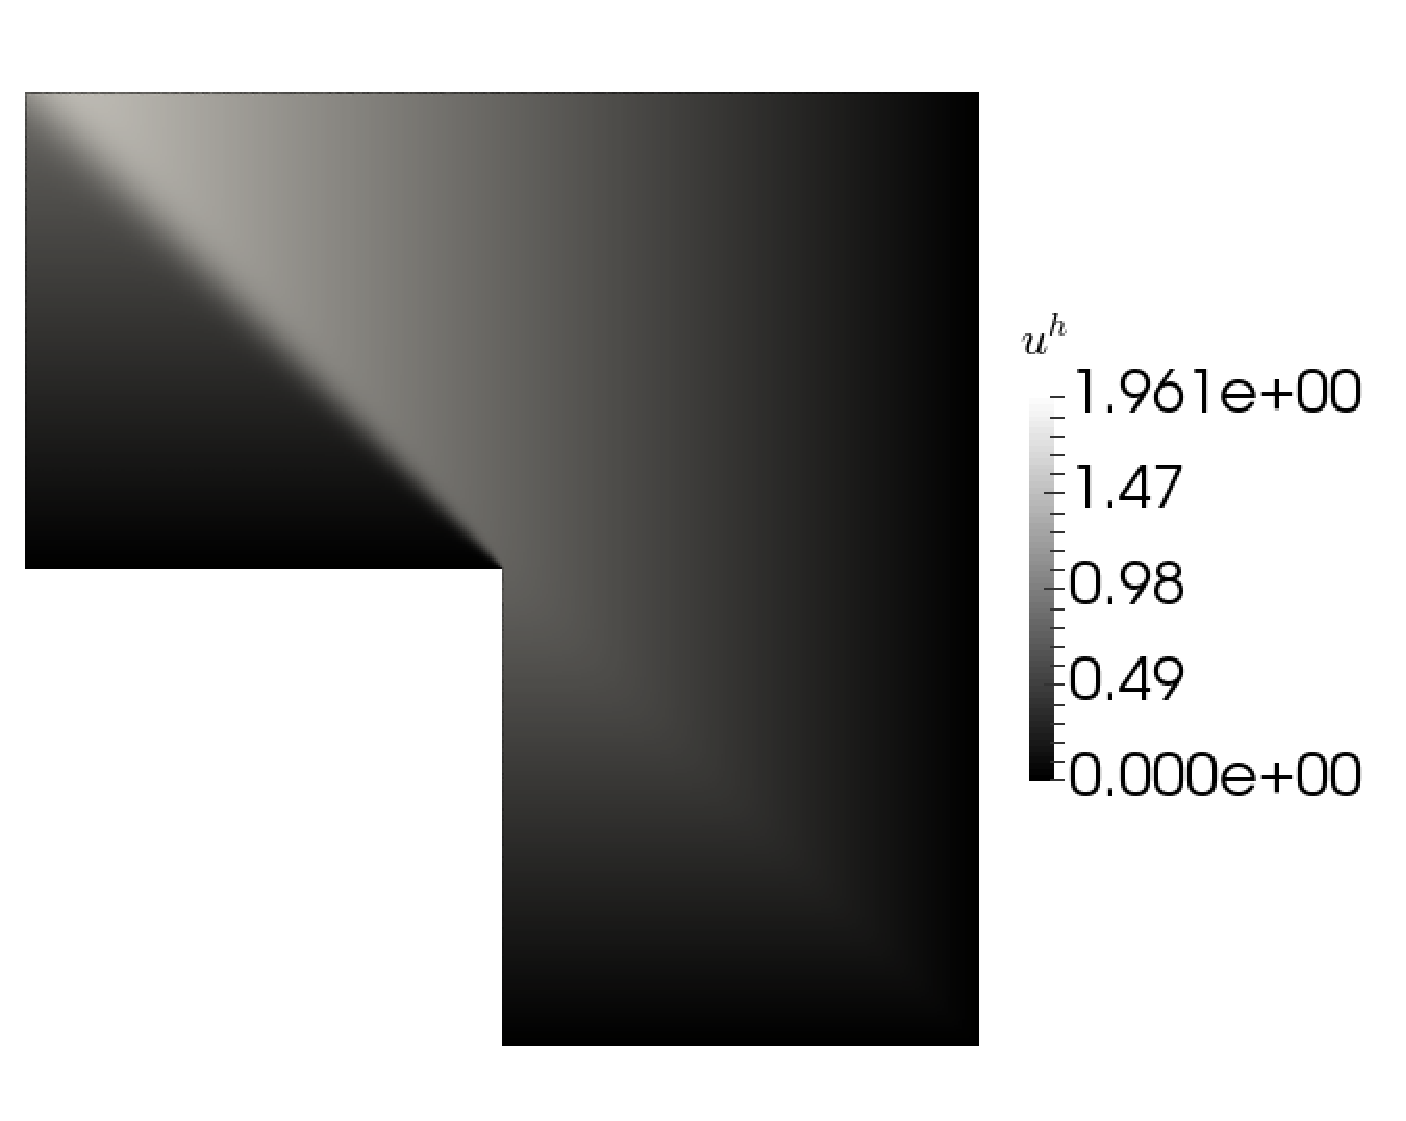
\includegraphics[width=.99\linewidth]{img/vms_lshape_uh}
\end{subfigure}%
\begin{subfigure}{.3\textwidth}
\centering
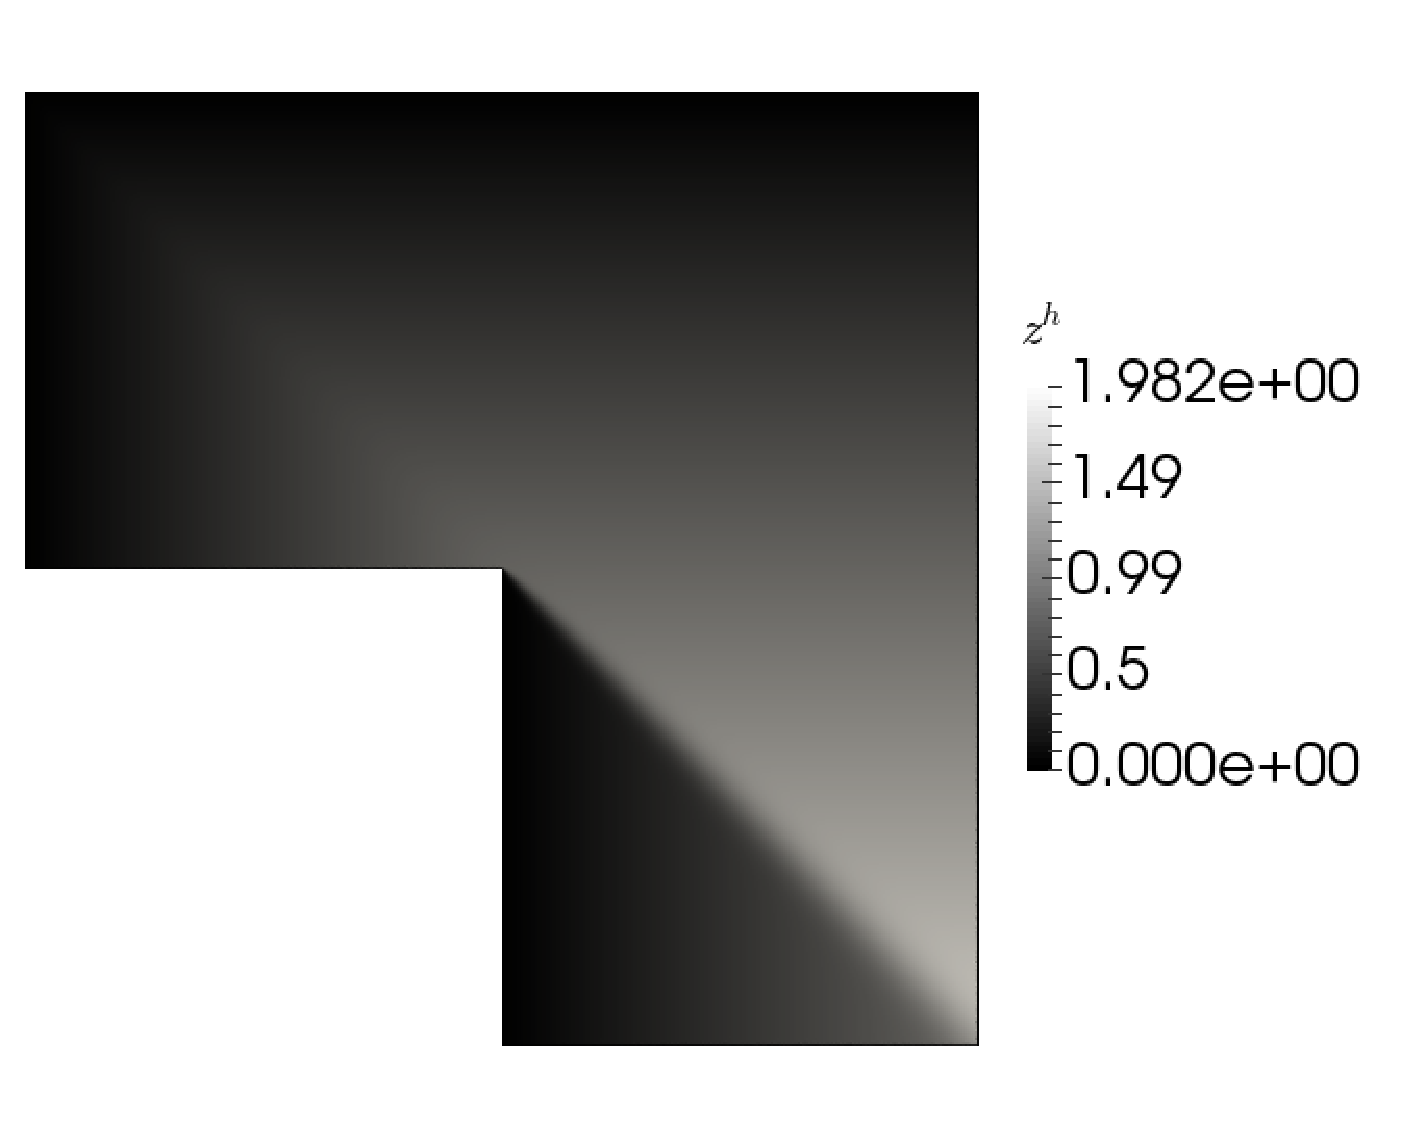
\includegraphics[width=.99\linewidth]{img/vms_lshape_global_zh}
\end{subfigure}%
\begin{subfigure}{.3\textwidth}
\centering
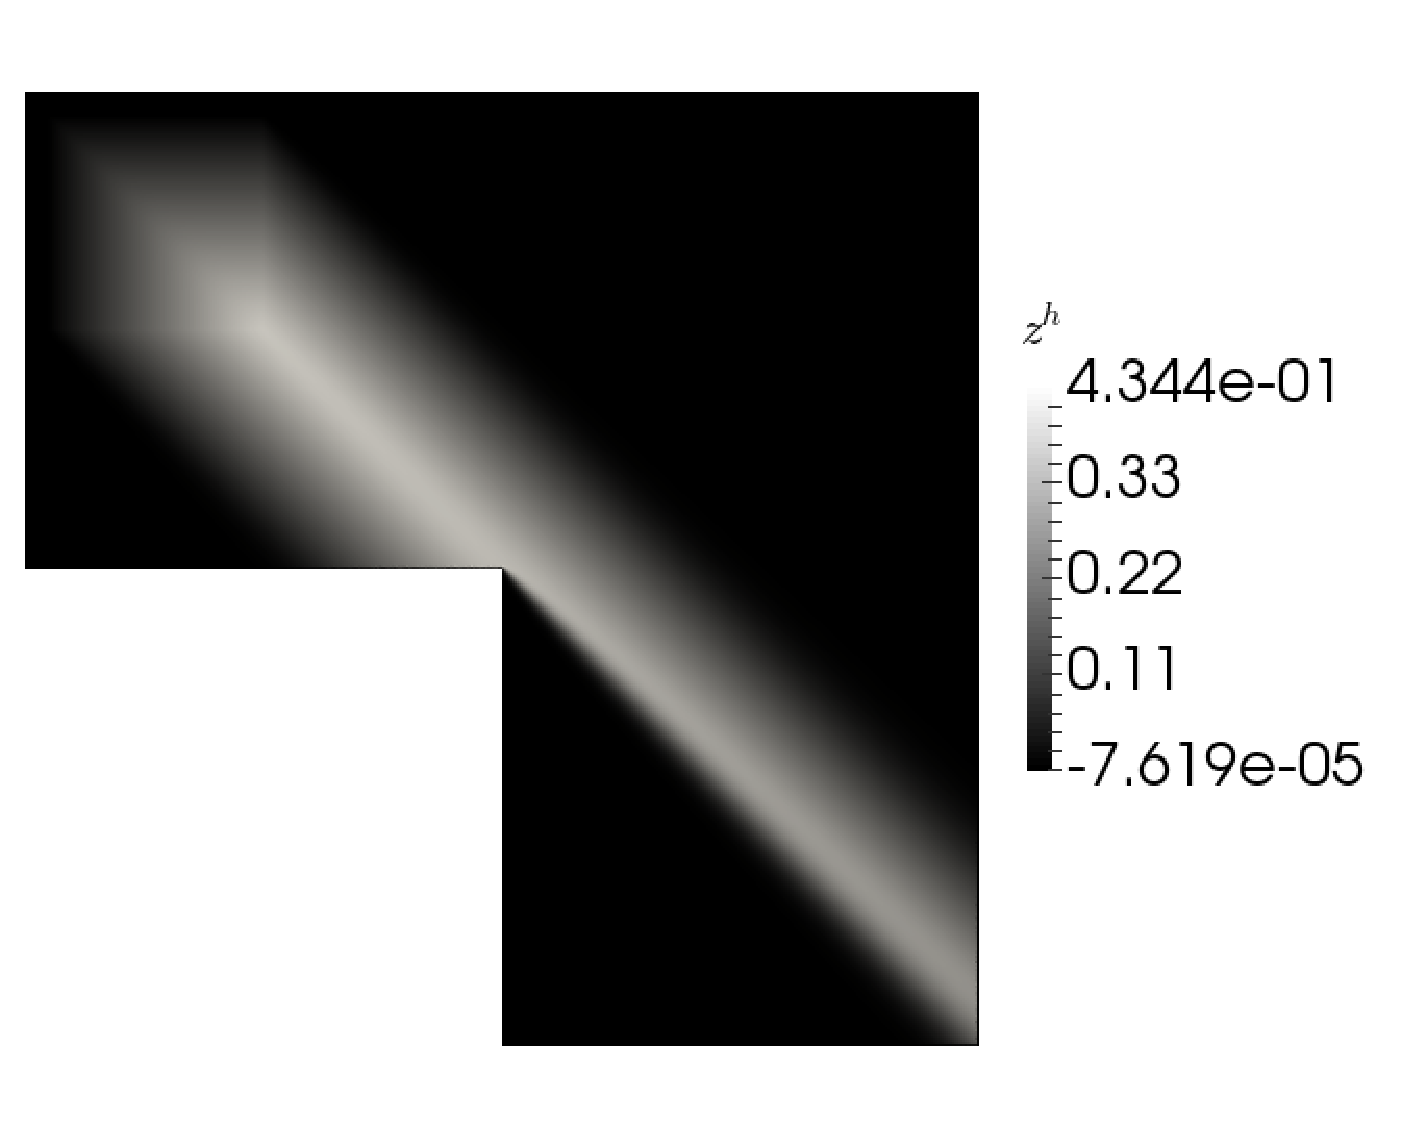
\includegraphics[width=.99\linewidth]{img/vms_lshape_square_zh}
\end{subfigure}
\caption{The primal solution $u^h$ (left) and the dual
solutions $z^h$ corresponding to $J_1(u)$ (center)
and $J_2(u)$ (right)}
\label{fig:lshape_solutions}
\end{figure}

We investigate the ability of four adaptive schemes
to accurately assess the two functional quantities.
Each scheme proceeds by iteratively performing the
steps
%
\begin{gather*}
\text{Solve primal PDE} \rightarrow
\text{Localize error} \rightarrow
\text{Adapt mesh}.
\end{gather*}
%
The first adaptive scheme, referred to as
\textsc{UNIF}, remeshes the entire domain
with a uniform size field. For the two output quantities,
errors are computed for the meshes generated with the
mesh sizes
$h = \{ \frac{1}{4}, \frac{1}{8}, \frac{1}{16},
\frac{1}{32}, \frac{1}{64} \}$. In principle, the
step to localize the error is not required for this
scheme.

For comparison to more traditional energy-based methods,
the second adaptive scheme is chosen based
on a Zienkiewicz-Zhu type error estimate
\cite{zienkiewicz1992superconvergenti}
\cite{zienkiewicz1992superconvergentii},
whereby error indicators are computed as the difference
between solution gradients $\nabla u^h$ that are
discontinuous between elements and a nodally
smoothed approximation to the gradient
$(\nabla u^h)^*$ that is obtained via a
least-squares fit over a patch of elements.
Once error indicators are computed,
the size field is set according to the size
field equation \eqref{eq:size} such that the
target number of elements $N$ is twice the number
of elements in the previous mesh.
We refer to this scheme as the superconvergent
patch recovery (\text{SPR}) adaptive scheme.

The third and fourth adaptive schemes are based on the
error indicators $\eta^e_1$ and $\eta^e_2$, respectively,
and are referred to as the \textsc{VMS1} and \textsc{VMS2}
adaptive schemes, respectively. Again, once the error
indicators have been computed, the size field is set
according to the size field equation \eqref{eq:size}
such that the target number of elements $N$ is twice
the number of elements in the previous mesh.
We note that the scheme \textsc{VMS2} is the only one
which necessitates the solution of the dual PDE model,
which is implicitly included in the `Localize error'
step.

\begin{figure}[hbt!]
\centering
\begin{subfigure}{.3\textwidth}
\centering
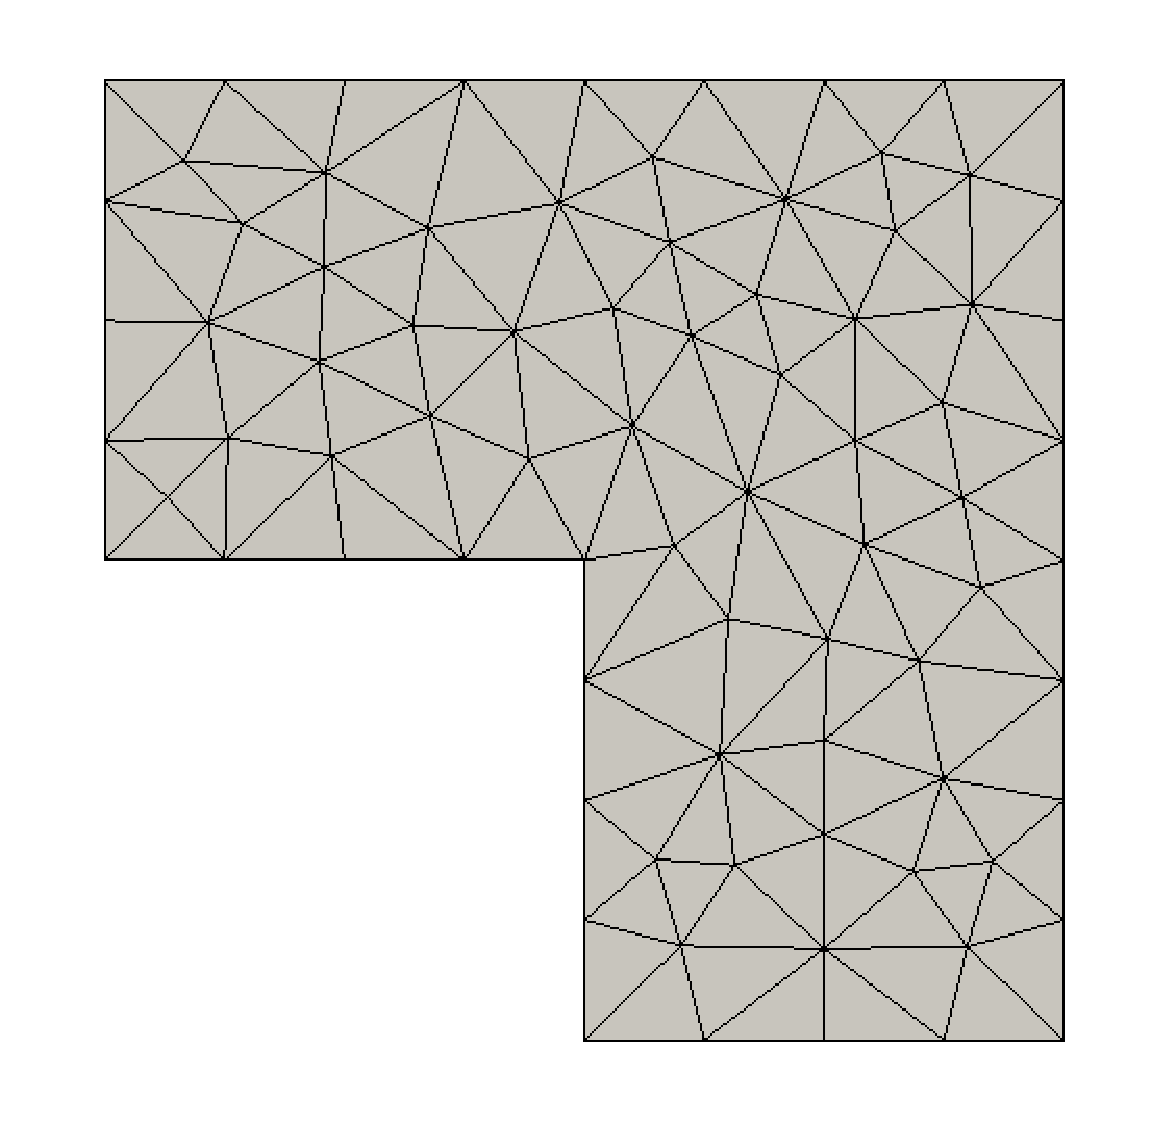
\includegraphics[width=.99\linewidth]{img/vms_lshape_global_initial}
\end{subfigure}%
\begin{subfigure}{.3\textwidth}
\centering
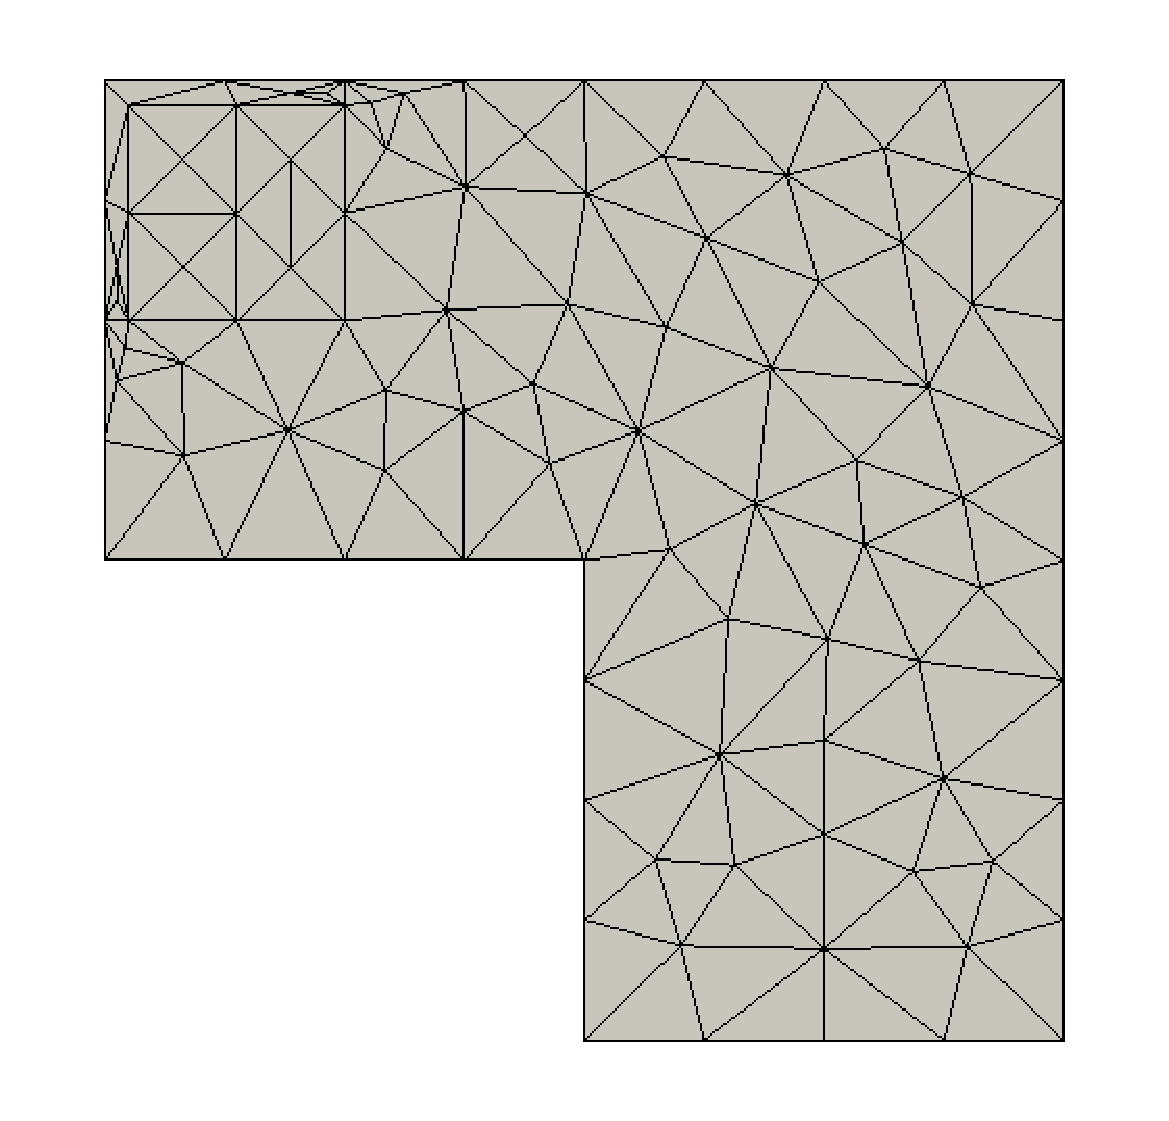
\includegraphics[width=.99\linewidth]{img/vms_lshape_square_initial}
\end{subfigure}%
\caption{Initial meshes for the outputs $J_1(u)$ (left) and $J_2(u)$ (right)}
\label{fig:global_meshes}
\end{figure}

For each quantity of interest, an initial mesh with
a uniform size of $h=\frac{1}{4}$ was generated as
shown in Figure \ref{fig:global_meshes}. From this
initial mesh, each adaptive scheme was run until
meshes with over $10,000$ degrees of freedom were
produced. The exact values of the two output quantities
were computed on `truth' meshes, which are finer
at every spatial location in the domain when compared
to the meshes obtained via the four adaptive schemes.
The values of the  quantities of interest were found to be
$J_1(u) = 1.6588688371$ and $J_2(u) = 0.23109653499$.

\begin{figure}[hbt!]
\centering
\begin{subfigure}{.3\textwidth}
\centering
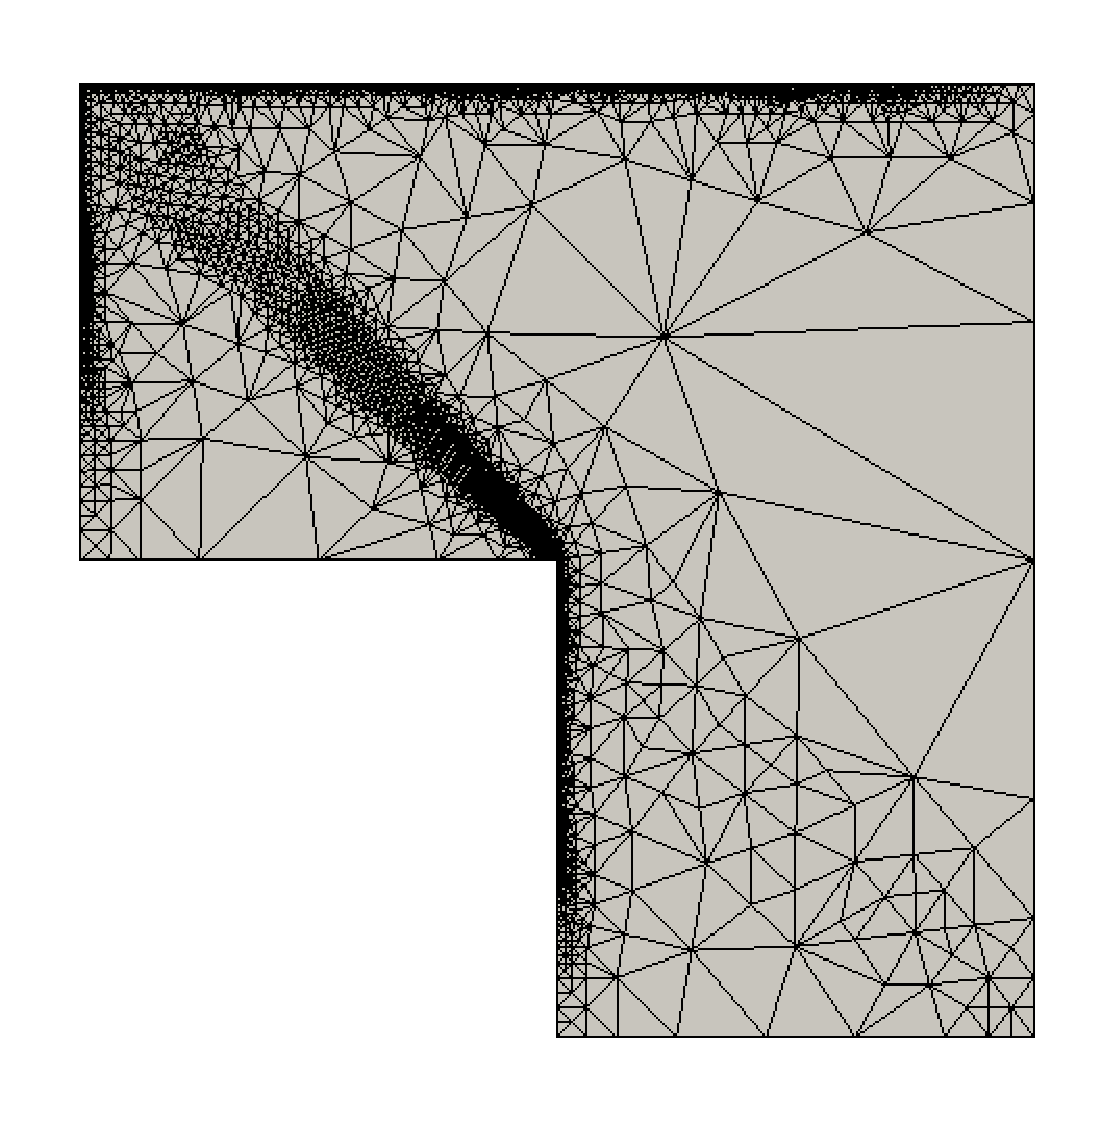
\includegraphics[width=.99\linewidth]{img/vms_lshape_global_spr_final}
\end{subfigure}%
\begin{subfigure}{.3\textwidth}
\centering
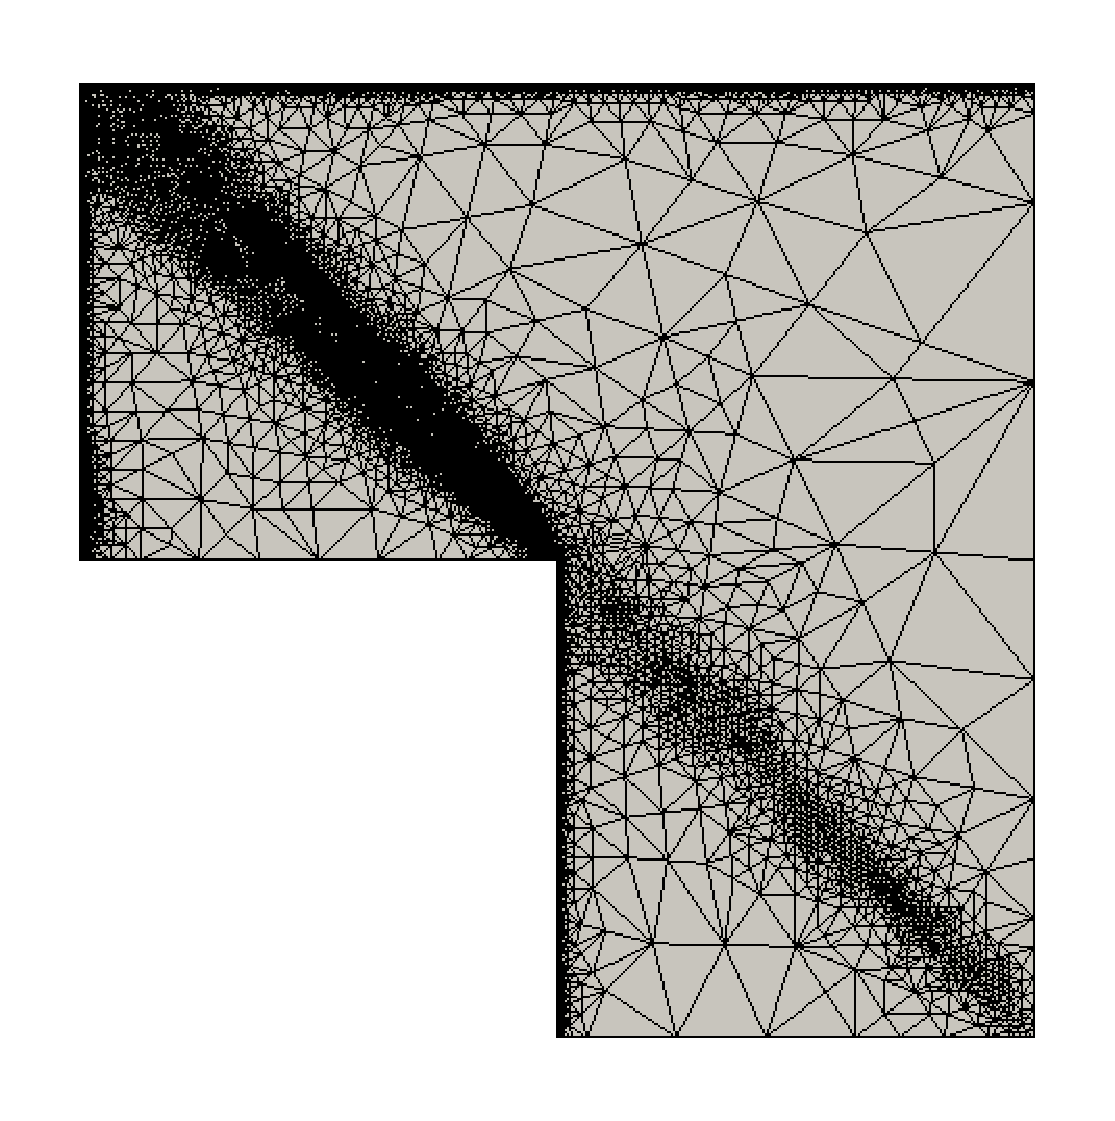
\includegraphics[width=.99\linewidth]{img/vms_lshape_global_vms1_final}
\end{subfigure}%
\begin{subfigure}{.3\textwidth}
\centering
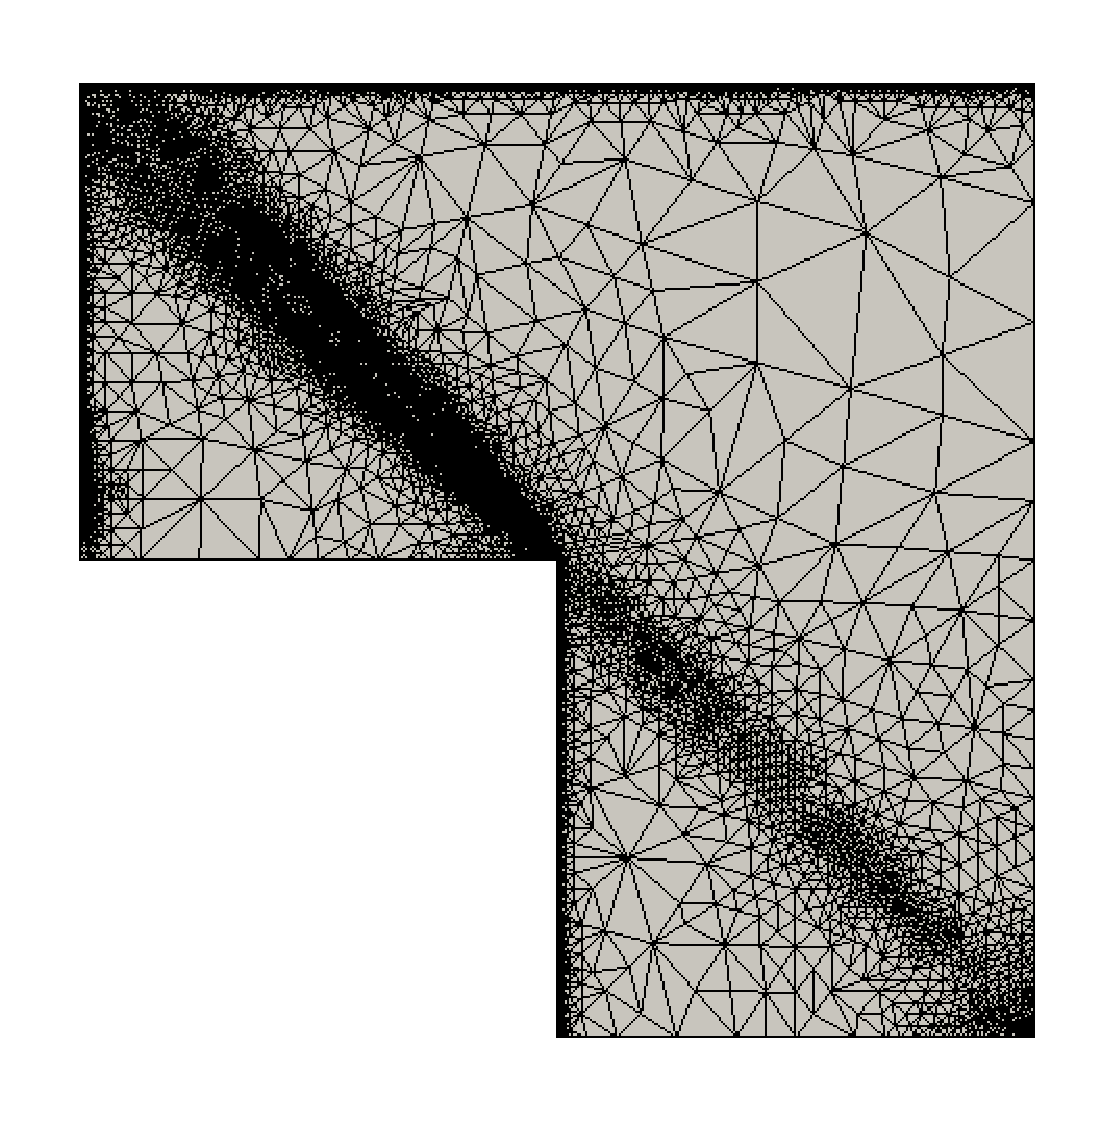
\includegraphics[width=.99\linewidth]{img/vms_lshape_global_vms2_final}
\end{subfigure}
\caption{Final adapted meshes for the output $J_1(u)$ using
the SPR (left), VMS1 (center), and VMS2 (right) adaptive schemes}
\label{fig:J1_meshes}
\end{figure}

\begin{figure}[hbt!]
\centering
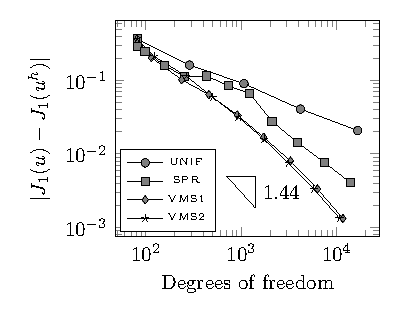
\includegraphics[width=.5\linewidth]{img/vms_lshape_global_convergence}
\caption{Convergence history for various adaptive schemes for
the output $J_1(u)$.}
\label{fig:J1_convergence}
\end{figure}

Figure \ref{fig:J1_meshes} shows the meshes obtained at the
final iteration of the \textsc{SPR}, \textsc{VMS1}, and
\textsc{VMS2} adaptive schemes for the global output quantity
$J_1(u)$. As expected, the \textsc{SPR} scheme strongly refines
the mesh in areas where the gradient changes drastically.
These areas include the left-most and upper-most surfaces
of the L-shaped domain where boundary layers in the solution
exist, as well as the diagonal downstream of the
reentrant corner where there is a sudden change in the
solution magnitude. In addition to performing mesh refinement
in the areas that the \textsc{SPR} scheme targets, the
\textsc{VMS1} and \textsc{VMS2} also refine the mesh along
the diagonal upstream of the reentrant corner to accurately
resolve features of the dual solution $z^h$. For the global
quantity $J_1(u)$, the \textsc{VMS1} and \textsc{VMS2}
schemes yield final meshes with very similar characteristics.
At each iteration in the adaptive schemes, the
output error $|J_1(u) - J_1(u^h)|$ was computed.
Figure \ref{fig:J1_convergence} displays the convergence
histories for each adaptive scheme. Unsurprisingly,
the \textsc{VMS1} and \textsc{VMS2} adaptive schemes
compute the output error more accurately than the
\textsc{SPR} and \textsc{UNIF} with a comparable number
of degrees of freedom.

\begin{figure}[hbt!]
\centering
\begin{subfigure}{.3\textwidth}
\centering
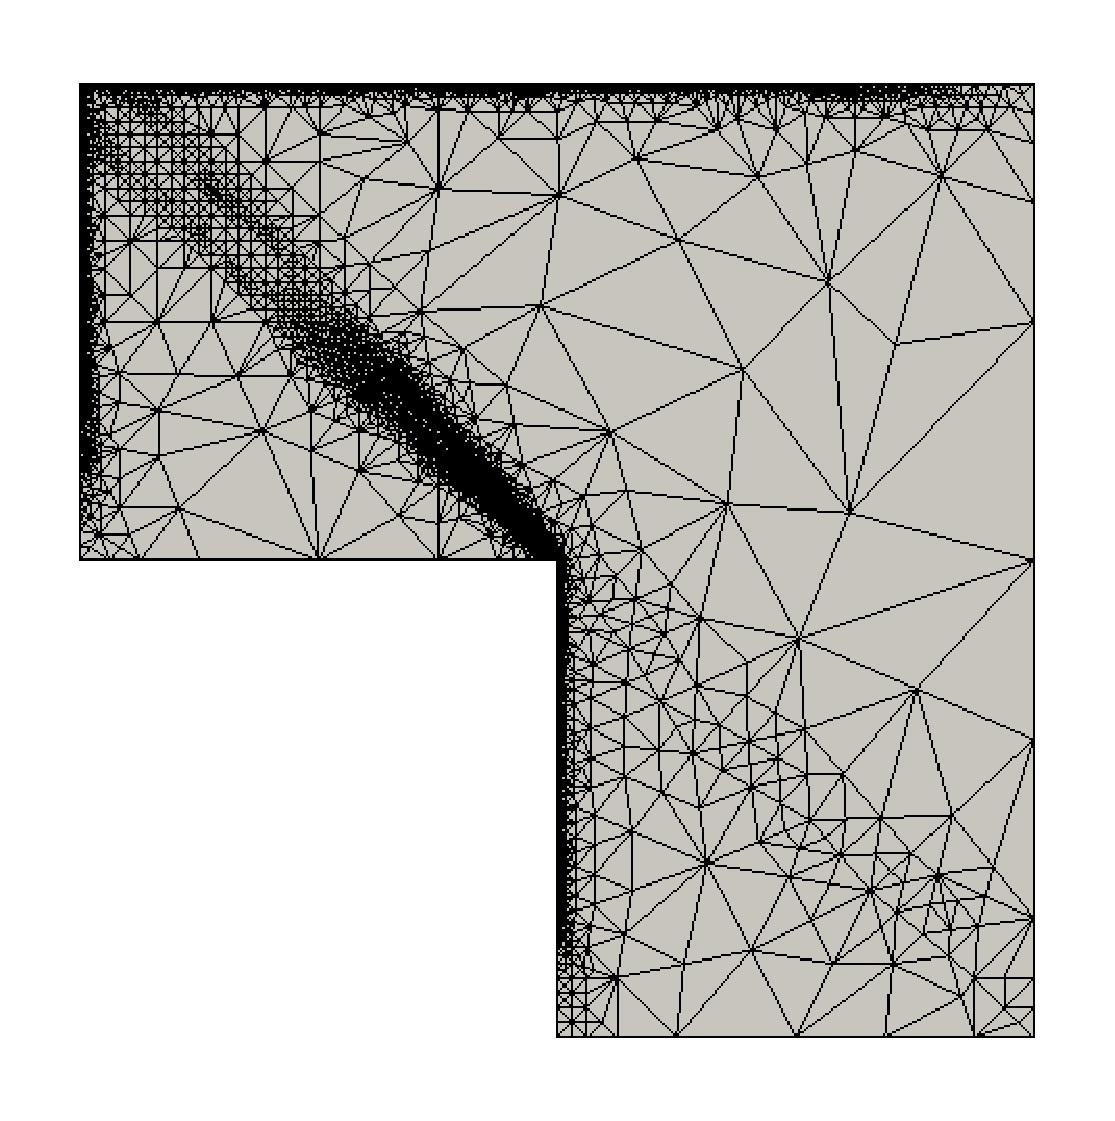
\includegraphics[width=.99\linewidth]{img/vms_lshape_square_spr_final}
\end{subfigure}%
\begin{subfigure}{.3\textwidth}
\centering
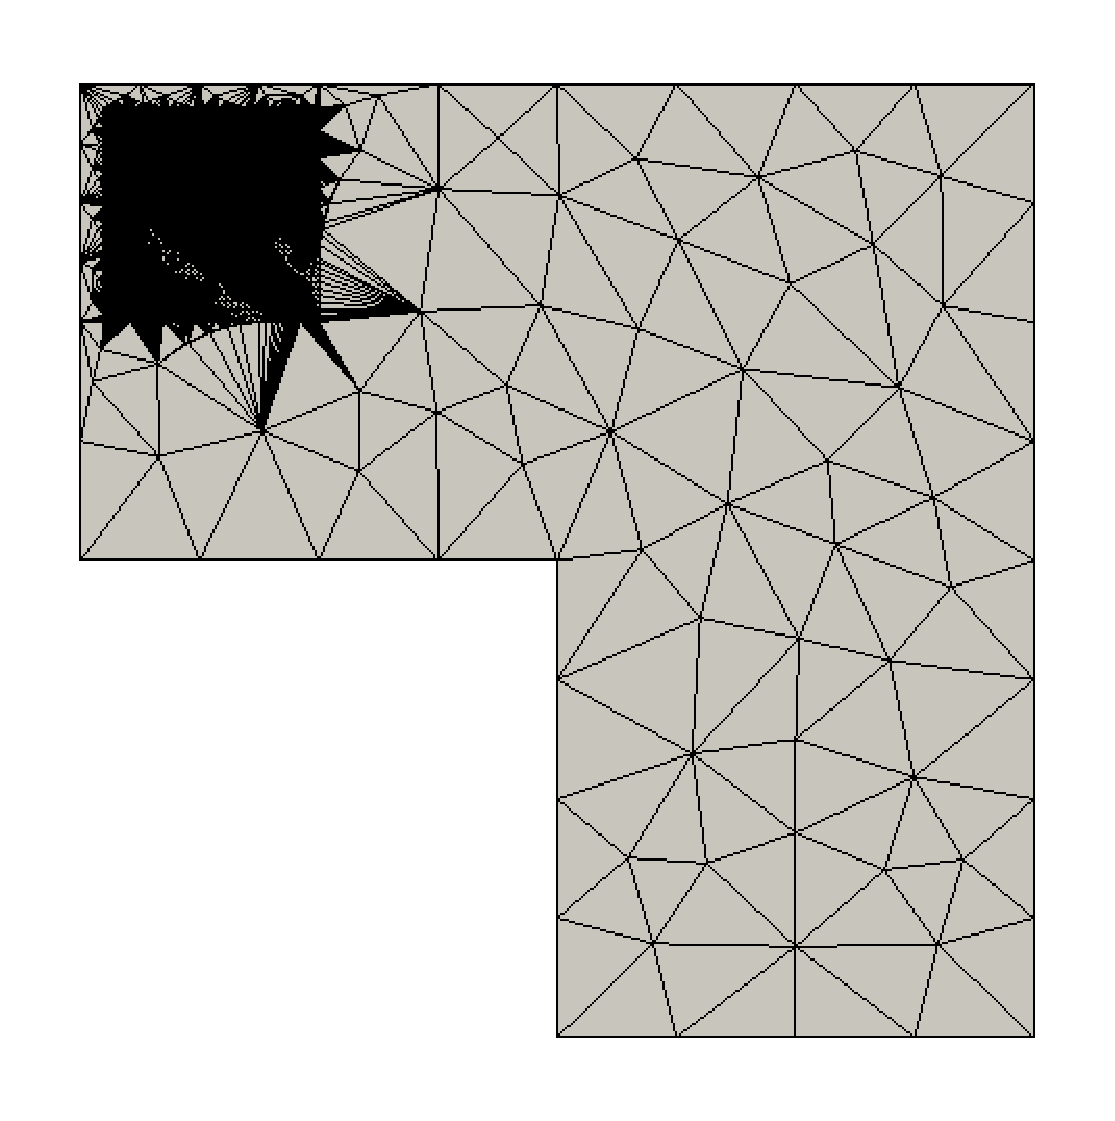
\includegraphics[width=.99\linewidth]{img/vms_lshape_square_vms1_final}
\end{subfigure}%
\begin{subfigure}{.3\textwidth}
\centering
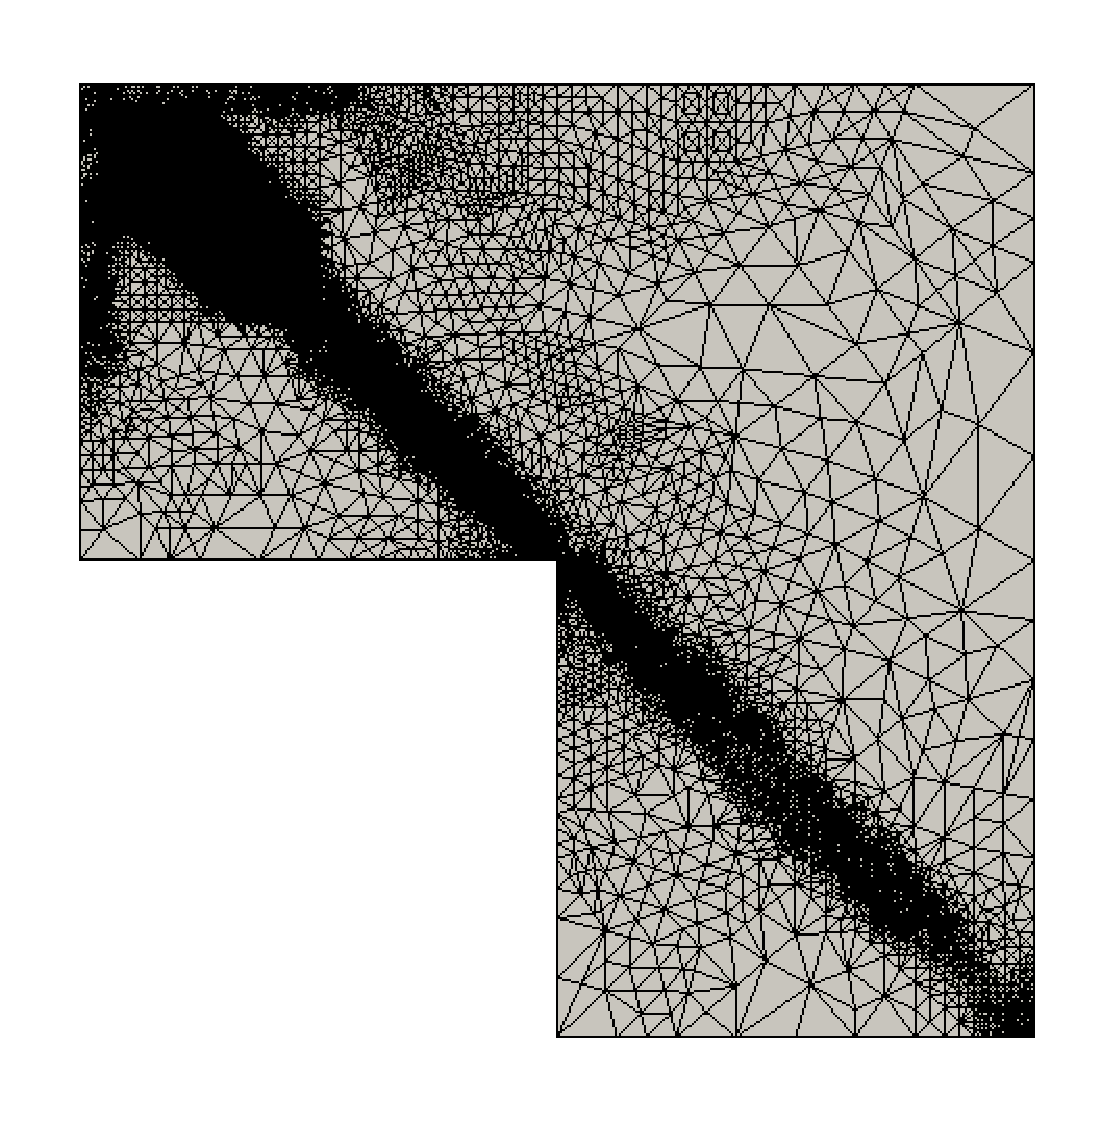
\includegraphics[width=.99\linewidth]{img/vms_lshape_square_vms2_final}
\end{subfigure}
\caption{Final adapted meshes for the output $J_2(u)$ using
the SPR (left), VMS1 (center), and VMS2 (right) adaptive schemes}
\label{fig:J2_meshes}
\end{figure}

\begin{figure}[hbt!]
\centering
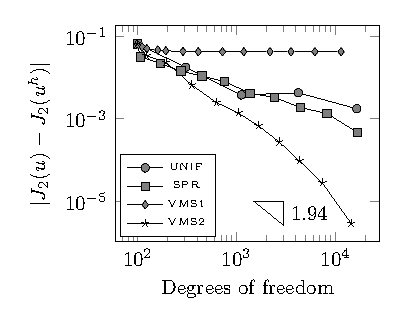
\includegraphics[width=.5\linewidth]{img/vms_lshape_square_convergence}
\caption{Convergence history for various adaptive schemes for
the output $J_2(u)$.}
\label{fig:J2_convergence}
\end{figure}

Figure \ref{fig:J2_meshes} displays the output meshes at
the final iteration of the \textsc{SPR}, \textsc{VMS1},
and \textsc{VMS2} adaptive schemes for the local
output quantity $J_2(u)$. Again, it is clear that the
\textsc{SPR} strongly refines the mesh in areas where the
gradient changes drastically. The \textsc{VMS1} scheme
only performs mesh refinement over the square subdomain
over which $q_2$ is non-zero and does not seek
accurately resolve the mesh to capture features of
the primal or dual solutions. In contrast, the
\textsc{VMS2} strongly refines the mesh over the
square subdomain of interest, while also resolving
areas upstream of the domain to accurately account
for the features of the primal and dual solutions.
For the output quantity $J_2(u)$, convergence histories
for each adaptive scheme are shown in Figure
\ref{fig:J2_convergence}. It is clear from both
the convergence diagram and final adapted mesh
for the \textsc{VMS1} scheme that the \textsc{VMS1}
scheme is completely insufficient to drive mesh
adaptation for a locally defined output quantity.
On the other hand, the \textsc{VMS2} adaptive scheme
is able to compute the ouptut quantity with much
greater accuracy than the \textsc{UNIF} and
\textsc{SPR} schemes when using a comparable number
of degrees of freedom.

%%%%%%%%%%%%%%%%%%%%%%%%%%%%%%%%%%%%%%%%%%%%%%%%%%%%%%%%%%%%%%%%%%%%%%%%%%%%%%
\section{Conclusions}
%%%%%%%%%%%%%%%%%%%%%%%%%%%%%%%%%%%%%%%%%%%%%%%%%%%%%%%%%%%%%%%%%%%%%%%%%%%%%%

For VMS methods, we have proposed a novel approach
to enriching the dual solution for duality-based
functional error estimation using VMS techniques.
We have demonstrated the utility of this technique
to drive mesh adaptation to accurately compute
output quantities.

Future work includes investigating the effect
of choosing different optimality conditions
$\phi(\cdot)$ and $\phi_d(\cdot)$ for the primal
and dual problems, respectively, extending
error estimates to account for nonlinearities
in both the PDE model and in the functional output
quantity, investigating the effect of
utilizing more accurate approximations to the
fine-scale primal and dual solutions, and
extending the arguments presented to
a mixture of non-homogeneous Dirichlet
and Nuemann boundary conditions.
